% Relatório da versão 1 do software ipump para o curso
% Sistemas de Controle - DCA0206 - UFRN
% Autores:
%   AUGUSTO MATHEUS PINHEIRO DAMASCENO
%   MARCEL DA CÂMARA RIBEIRO DANTAS
%   PABLO HOLANDA CARDOSO
%   PEDRO DE CASTRO GURGEL LIMA
%   RODRIGO DANTAS DA SILVA
% Modificado por: Ícaro Bezerra Queiroz de Araújo
%

%%%%%%%%%%%% STRUCTURE %%%%%%%%%%%%%%%
\documentclass[a4paper,12pt]{article}
\usepackage[T1]{fontenc}
\usepackage[utf8]{inputenc}
\usepackage[brazil]{babel}
\usepackage{lmodern}
\usepackage{setspace}
\usepackage[top=2cm, bottom=2cm, left=2cm, right=2cm]{geometry}
%%%%%%%%%%%%%%%%%%%%%%%%%%%%%%%%%%%%%%

%%%%%%%%%%%%%%%% PAGES STYLE %%%%%%%%%
\usepackage{fancyhdr}
\fancypagestyle{main}{
\renewcommand{\headrulewidth}{0pt}
\fancyhead[RO]{\thepage}
\fancyfoot[CO]{}
}
%%%%%%%%%%%%%%%%%%%%%%%%%%%%%%%%%%%%%%

\usepackage{graphicx}
\usepackage{float}
\usepackage{epstopdf}
\usepackage{subfig}
\usepackage{mathptmx}
\usepackage{changepage}


\usepackage{listings}
\usepackage{xcolor}
\lstset{language=C++,
                basicstyle=\ttfamily,
                keywordstyle=\color{blue}\ttfamily,
                stringstyle=\color{red}\ttfamily,
                commentstyle=\color{green}\ttfamily,
                morecomment=[l][\color{magenta}]{\#}
}

%\usepackage[alf]{abntex2cite}

%%%%%%%%%%% PDF METADATA %%%%%%%%%%%%%
\usepackage[ pdftitle={MODELO RELATÓRIO},
pdfsubject={INTRODUÇÃO AO LABORATÓRIO DE CONTROLE - Grupo 3},
pdfkeywords={Controle,Automação,UFRN,DCA,ipump},
hidelinks]{hyperref}
%%%%%%%%%%%%%%%%%%%%%%%%%%%%%%%%%%%%%%

\begin{document}

\onehalfspacing

\thispagestyle{empty}

\setcounter{page}{1}

%%%%%%%%%%%% LOGOS %%%%%%%%%%%%%%%%%%%

\begin{figure}[!ht]

\centering

\subfloat{

\includegraphics[width=2.7cm]{UFRN.eps}
\label{UFRN Logo}
}
\hspace{11.09cm}
\subfloat{

\includegraphics[width=2.4cm]{DCA.eps}
\label{DCA Logo}
}

%\caption{}
\label{Logos}

\end{figure}

%%%%%%%%%%%%%%% CAPA %%%%%%%%%%%%%%%%%

\vspace{-1cm}

\begin{center}
{\bf{\normalsize UNIVERSIDADE FEDERAL DO RIO GRANDE DO NORTE\\
CENTRO DE TECNOLOGIA\\
DEPARTAMENTO DE ENGENHARIA DE COMPUTAÇÃO E AUTOMAÇÃO\\
CURSO DE ENGENHARIA DE COMPUTAÇÃO
}}


\vspace{3.6cm}

{\bf{\large RELATÓRIO DA 4ª EXPERIÊNCIA\\
CONTROLE DE SISTEMAS DINÂMICOS: CONTROLE EM CASCATA\\
}}
\vspace{1.5cm}
{\large TURMA: 01 A\\
	GRUPO Nº 02}


\vspace{3.6cm}


\begin{flushright}
\begin{normalsize}
ANDRESSA STÉFANY SILVA DE OLIVEIRA: 20160154101\\
\vspace{0.8cm}
FERNANDA MONTEIRO DE ALMEIDA: 20160154228\\
\vspace{0.8cm}
MÁRCIO LUIZ BEZERRA LOPES JÚNIOR: 20160154326\\
\vspace{0.8cm}
VITOR RAMOS GOMES DA SILVA: 20160154415\\
\end{normalsize}
\end{flushright}


\vspace{2.5cm}

{\large Natal-RN\\
2017}

\end{center}

\newpage

%%%%%%%%%%%%%%%  CONTRA-CAPA %%%%%%%%%

\thispagestyle{empty}

\begin{center}
\begin{normalsize}
ANDRESSA STÉFANY SILVA DE OLIVEIRA: 2016015410\\
\vspace{0.8cm}
FERNANDA MONTEIRO DE ALMEIDA 20160154228\\
\vspace{0.8cm}
MÁRCIO LUIZ BEZERRA LOPES JÚNIOR: 20160154326\\
\vspace{0.8cm}
VITOR RAMOS GOMES DA SILVA: 20160154415\\

\end{normalsize}
\end{center}
\vspace{3cm}

{\bf{\large {\centering CONTROLE DE SISTEMAS DINÂMICOS: CONTROLE EM CASCATA\\}}}

\vspace{4cm}

\begin{adjustwidth}{7.5cm}{0cm}

{\normalsize
Quarto Relatório apresentado à disciplina de
Laboratório de Sistemas de Controle, correspondente à
avaliação da 2º unidade do semestre 2017.1 do 8º período
do curso de Engenharia de Computação da
Universidade Federal do Rio Grande do Norte, sob
orientação do {\bf Prof. Fábio Meneghetti Ugulino de
Araújo} e {\bf Prof. Lucas Costa Pereira Cavalcante.}

}

\end{adjustwidth}

\vspace{2cm}

\begin{center}

Professores:  Fábio Meneghetti Ugulino de Araújo e\\
Lucas Costa Pereira Cavalcante.

\vspace{2.5cm}

{\large Natal-RN\\
2017}

\end{center}

\newpage

%%%%%%%%%%%%%%%  RESUMO %%%%%%%%%%%%%%

\thispagestyle{empty}

\begin{center}
{\large \textbf{RESUMO}}
\end{center}

\vspace{3cm}

\begin{flushleft}

\hspace{4ex}O presente trabalho é a quarta etapa da construção de um aplicativo desktop para controle de sistema de tanques. O software utiliza a comunicação cliente/servidor no qual o sistema de tanques é o servidor. A planta antes utilizada da Quanser foi substituída por uma simulação feita em Java3D, o que eliminou o nível de ruído dos resultados. Nesta etapa do trabalho, o objetivo foi a implementação de controladores P, PI, PD, PID e PI-D de segunda ordem na configuração controle em cascata. A teoria acerca de controle em cascata é introduzida, após é apresentado os resultados dos testes de controle da planta. Por fim, chega-se a conclusão que o controle em cascata tem uma resposta mais rápida em relação às pequenas modificações de nível, mas não tendo a sintonização correta se perde as vantagens adquiridas. \\

\end{flushleft}

\vspace{1.5cm}

\textbf{Palavras-chave:} sistema de tanques; sistema de controle; software; planta Quanser, controlador PID; controle em cascata.

\newpage

%%%%%%%%% LISTA DE FIGURAS %%%%%%%%%%%

\thispagestyle{empty}

\begin{center}
\listoffigures
\end{center}

\newpage

%%%%%%%%%%%%%%% SUMÁRIO %%%%%%%%%%%%%%

\thispagestyle{empty}

\begin{center}
\tableofcontents
\end{center}

\newpage

%%%%%%%%%%%%%%% INTRODUÇÃO %%%%%%%%%%%

\thispagestyle{main}

\section{INTRODUÇÃO}

%\begin{flushleft}
\hspace{4ex}A prática de laboratório 04 tem como objetivo introduzir um sistema de controle em cascata na planta \textit{Quanser}, sendo a figura \ref{r2d2e} o simulador da planta:

\begin{figure}[H]
\centering
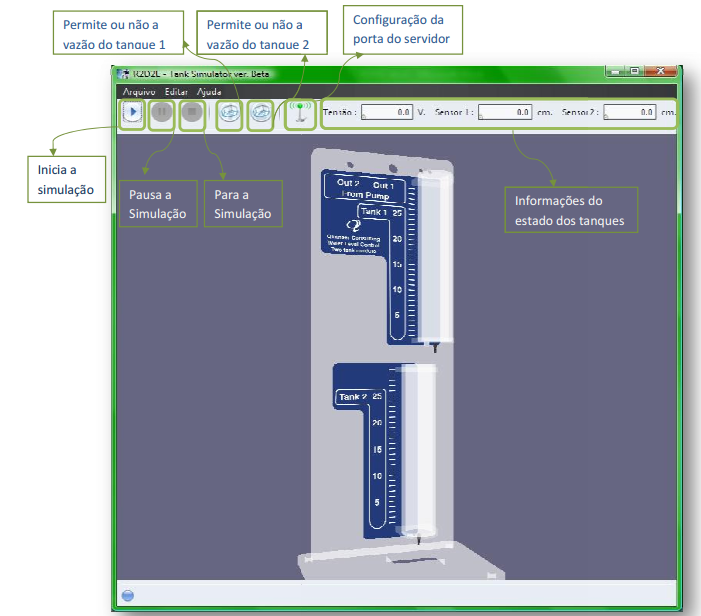
\includegraphics[width=11cm]{ImagensLab4/simulator.png}
\caption{R2D2E - Tank Simulator}
\label{r2d2e}
\end{figure}

\hspace{4ex}Pretende-se controlar o nível de água de ambos os tanques da planta, para isso, foi implementado os controladores Proporcional (P), Proporcional Integrativo (PI), Proporcional Derivativo (PD), Proporcional Integrativo Derivativo (PID) e Proporcional Integrativo Derivativo em controle de ação baseado no sinal do processo (PI-D). Quem irá escolher qual controle será usado é o usuário, através da interface do programa desenvolvido, como mostrado na figura \ref{interface}:

\begin{figure}[H]
\centering
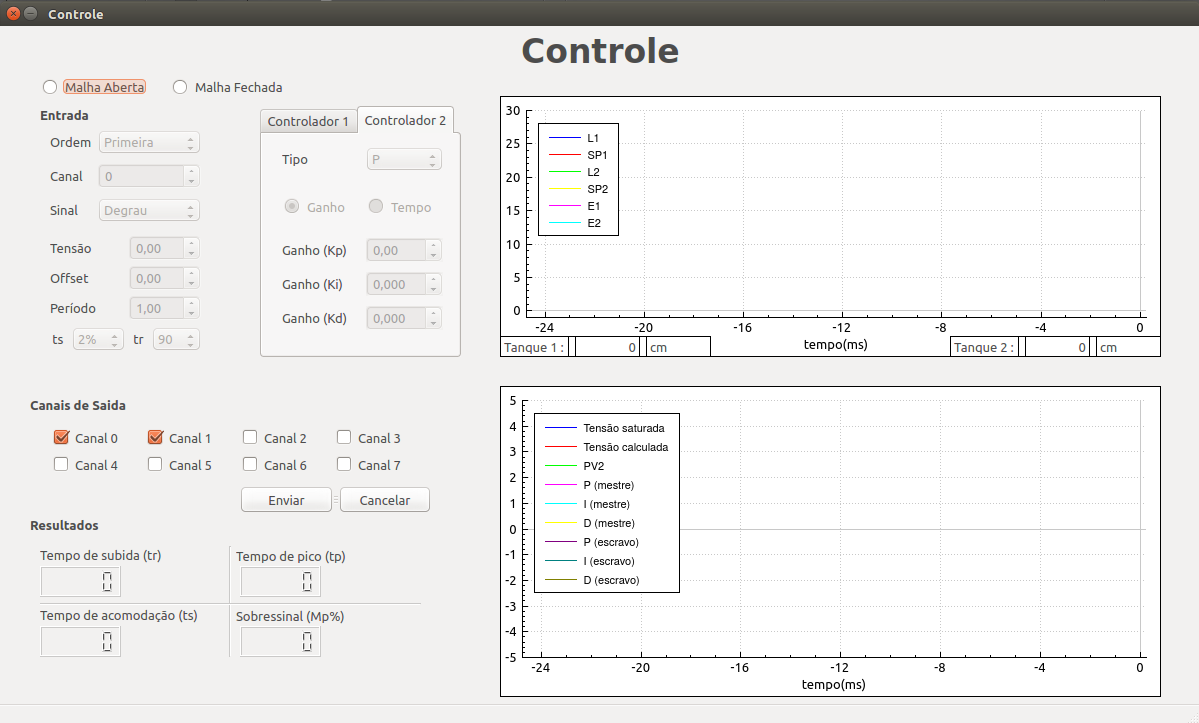
\includegraphics[width=11cm]{ImagensLab4/interface-versao4.png}
\caption{Interface do software de controle}
\label{interface}
\end{figure}

\hspace{4ex}Além dessas opções, o usuário também deve escolher os ganhos dos controladores Kp, Ki e ou Kd, ou $\tau_i$ e $\tau_d$, os quais são necessários para o controlador, como também, o  sinal de referência a ser enviado, o offset, a análise da resposta do sistema para o tempo de subida (t$_r$), por exemplo, de 5\% à 95\%, e o tempo de acomodação (t$_s$), para as faixas de 2\%, 5\% e 10\% do degrau. Ademais, é possível saber os valores do  t$_r$, t$_s$, tempo de pico (t$_p$) e o sobressinal (Mp) do sistema de segunda ordem.

\hspace{4ex}O controle da planta se dará de duas formas: utilizando apenas uma malha de controle, como também, o controle em cascata. A configuração da planta mostrada na figura \ref{r2d2e} fazendo uso do controle de uma malha será da seguinte maneira:

\begin{figure}[H]
\centering
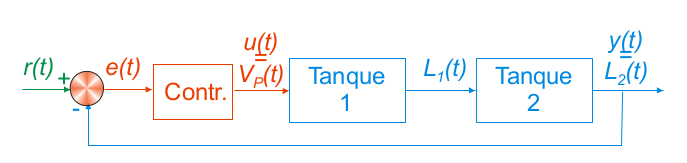
\includegraphics[width=11cm]{ImagensLab4/umamalha.png}
\caption{Configuração da planta utilizando uma malha de controle.}
\label{umamalha}
\end{figure}

\hspace{4ex}No caso mostrado acima, na figura \ref{umamalha}, a tensão enviada para a bomba está sendo manipulada para o tanque de baixo da planta alcançar o nível desejado pelo usuário, isso é possível por causa da relação entre os dois tanques: a vazão de saída do tanque de cima é a vazão de entrada do tanque de baixo. Através do cálculo do erro do sinal de referência e a medição do segundo tanque será fornecida uma tensão que deixe o tanque de cima com um nível de água a qual levará o tanque de baixo para o valor desejado.

\hspace{4ex}Com a configuração de duas malhas de controle, ou seja, utilizando o controle em cascata, teremos a seguinte configuração:

\begin{figure}[H]
\centering
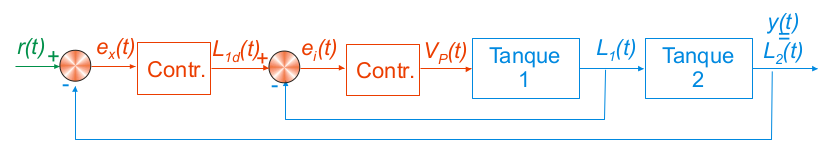
\includegraphics[width=11cm]{ImagensLab4/duasmalhas.png}
\caption{Configuração da planta utilizando o controle em cascata.}
\label{duasmalha}
\end{figure}

\hspace{4ex}Nesse caso, além de controlar o nível do tanque de baixo, pode-se controlar o nível do tanque de cima. Nessa configuração, denominamos o controlador mais externo de controlador mestre, o qual controla o nível do tanque de baixo da mesma forma que ocorre no controle com uma malha, e o controlador da malha interna é o controlador escravo, que a partir do erro entre o nível desejado do tanque de cima e seu nível real, irá determinar a tensão enviada para a bomba.

\hspace{4ex}No relatório é apresentado a metodologia utilizada nessa experiência, os resultados obtidos através de testes e as conclusões a partir da comparação do comportamento do sistema com uma e com duas malhas.

%\end{flushleft}

\newpage

%%%%%%%%%% REFERENCIAL TEÓRICO %%%%%%%

\thispagestyle{main}

\section{REFERENCIAL TEÓRICO}

\subsection{CONTROLE EM CASCATA}
\hspace{4ex}O controle em cascata é uma estratégia de controle que utiliza dois controladores aninhados de modo que a identificação de pequenos distúrbios aconteça de forma mais rápida e, consequentemente, a correção seja feita antes de o sistema sofrer grandes alterações. De forma genérica, o controle em cascata pode ser representando pelo diagrama da figura \ref{cascata}. Pode-se perceber que é necessário medir duas variáveis de processos, o da malha interna (chamada de malha escrava) e o da malha externa (chamada de malha mestre). Essas medidas, feitas através de uso de sensores, é comparada com a referência de cada malha. Sendo que a referência da malha externa, ou set point, é uma entrada do sistema. Já na malha interna, quem determina qual vai ser o "nível" a ser alcaçado é o controlador da malha externa. Então a malha do processo secundário recebe o erro, é feito o cálculo do nível para aquele processo que é enviado através de uma sinal de controle para o atuador, modificando o processo da malha interna.     

\begin{figure}[h]
\centering
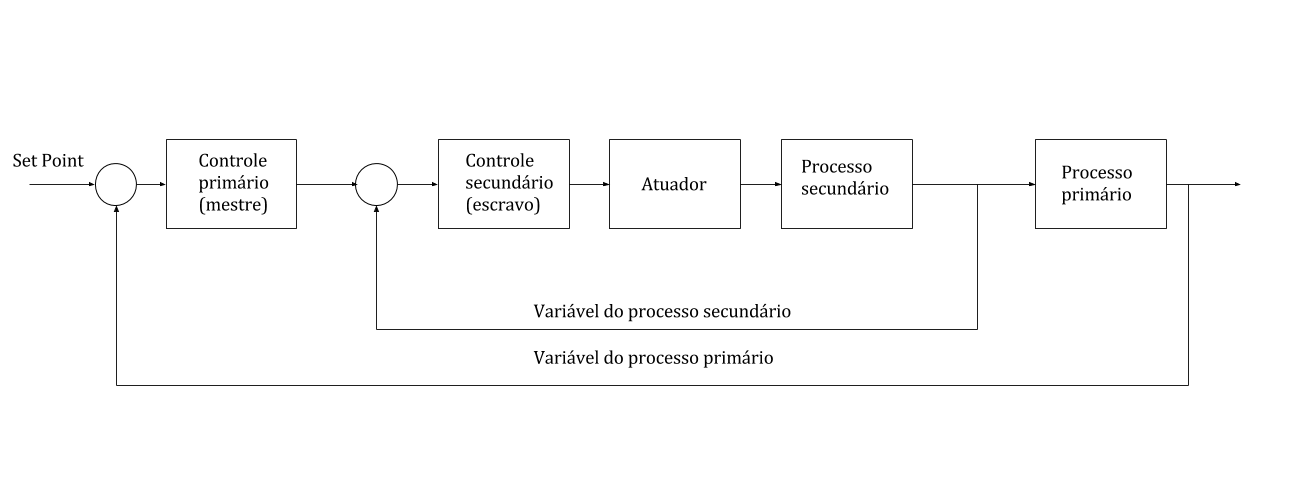
\includegraphics[width=17cm]{ImagensLab4/controle-em-cascata.png}
\caption{Diagrama de bloco do controle em cascata}
\label{cascata}
\end{figure}

Esse tipo de configuração é eficiente devido a dependência entre o processo primário e o secundário. Por exemplo, numa planta onde o gás que passa por um cano é resposável pelo aquecimento da água de um tanque, a atuação é feita controlando a quantidade de vazão do gás no cano. Há uma relação nesse processo em que quanto maior a vazão, mais quente ficará a água. Então a malha mestre seria o tanque com a água, e a malha escrava, a tubulação com gás. 

Outro aspecto importante a ser levado em consideração é a velocidade de cada processo. O processo primário tem que ser mais lento que o processo secundário. Como a temperatura varia de forma mais lenta que a vazão de um gás por uma tubulação, então não haveria conflito entre os sinais de controle. 

A questão de utilizar dois controladores vem dessa diferença de velocidades entre os processos, visto que uma diferença pequena de temperatura geraria um pequeno sinal de erro, logo, se tivesse apenas um controlador, o sinal enviado para controlar a vazão seria pequeno, o que não surtiria muito efeito na temperatura, quase não alteraria ou demoraria muito tempo. Já dois controladores conseguem mapear a relaçao entre o processo lento e um processo mais rápido. 

Uma das desvantagens de se utilizar o controle em cascata é que, ao adicionar mais um controlador, aumenta a complexidade de controle, pois é necessário sintonizar um quantidade dobrada de ganhos, gerando uma quantidade maior de combinações entre tipos de controle e ganhos possíveis. 




\newpage

%%%%%%%%%% METODOLOGIA %%%%%%%%%%%%%%%

\thispagestyle{main}

\section{METODOLOGIA}

\hspace{4ex}Utilizando o simulador R2D2E, foram feitos testes com o controlador mestre e o escravo, como também, com apenas um controlador para alcançar determinados níveis dos tanques da planta, os quais serão expostos nos resultados.

\hspace{4ex}Para isso, foi implementado uma classe controlador a qual é determinada de acordo com as escolhas do usuário, ou seja, se é P, PI, PD, PID ou PI-D. Por exemplo, se o usuário escolhe o controlador PD, ele fornecerá apenas os valores de Kp e Kd, ou Kp e $\tau_d$, e a partir desses valores a classe assumirá que Ki ou $\tau_i$ não existe, ou seja, o valor da integral será zero. O mesmo acontece se for escolhido o PI, nesse caso, o valor da derivada do erro será zero.

\hspace{4ex}Observe os métodos abaixo, o primeiro é para os casos em que o usuário escolher os controladores P, PI, PD ou PID, enquanto que o segundo método foi criado para o caso em que se quer usar o PI-D, pois utiliza o sinal do processo (y) ao invés de usar o erro.
\begin{lstlisting}
double PID::Controle(double e, double h)//Controladores P, PI, PD e PID
{
    I= I+Ki*e*h; //Simpsons (e+e_ant)*h/2 - integral do erro
    D= Kd*(e-e_ant)/h; //Derivada do erro
    e_ant= e; //Erro
    return Kp*e+I+D; //Sinal de controle
}

double PID::Controle(double e, double y, double h)//Controlador PI-D
{
    I= I+Ki*e*h; //Integral do erro
    D= Kd*(y-e_ant)/h; //Derivada do sinal do processo
    e_ant= y; //Sinal do processo
    return Kp*e+I+D; //Sinal de controle
}
\end{lstlisting}
\hspace{4ex}No software desenvolvido, esses valores podem ser escolhidos como mostrado na figura \ref{controladores}.

\begin{figure}[H]
     \centering
     \subfloat[][Controlador Mestre]{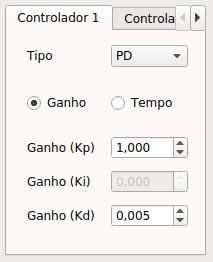
\includegraphics[width=4cm]{ImagensLab4/controlador1}\label{<figureP1>}}\hspace{4ex}
     \subfloat[][Controlador Escravo]{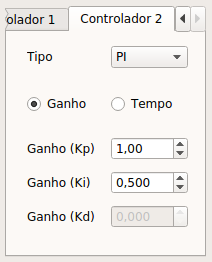
\includegraphics[width=4cm]{ImagensLab4/controlador2}\label{<figureP2>}}\\
     \caption{Interface para a escolha dos controladores}
     \label{fig:controladores}
\end{figure}


\newpage

%%%%%%%%%% RESULTADOS %%%%%%%%%%%%%%%

\thispagestyle{main}

\section{RESULTADOS}

\hspace{4ex}A análise do projeto desenvolvido foi realizada através da verificação das alterações do sistema quando testados diferentes valores e diferentes tipos de controladores.
Para o teste inicial, foram testados os controladores ambos com PIs de kp = 1 e ki = 0,03. Como pode ser observado na imagem a seguir (figura \ref{img1}), os níveis dos tanques (L1 e L2) ficaram bem abaixo do valor de finido de 10 cm e enquanto o nível no tanque 1 teve um tempo de subida inferior a 1s, o nível no tanque 2 teve um tempo de subida de quase 5s.
%img1

\begin{figure}[!h]
\centering
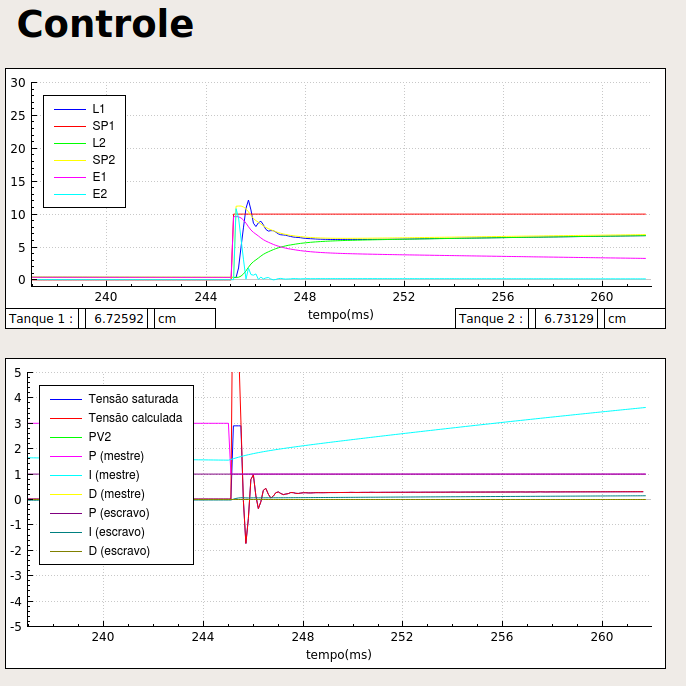
\includegraphics[width=11cm]{ImagensLab4/1.png}
\caption{Controle PI no mestre e no escravo}
\label{img1}
\end{figure}


No segundo teste foi aumentado o kp do controlador 1, de 1 para 3. O resultado percebido por essa alteração foi um nível em ambos os tanques mais próximo do esperado, um maior sobressinal para o tanque 1 e um tempo de subida consideravelmente mais alto para o tanque 2.
%[img0]
\newpage
\begin{figure}[!h]
\centering
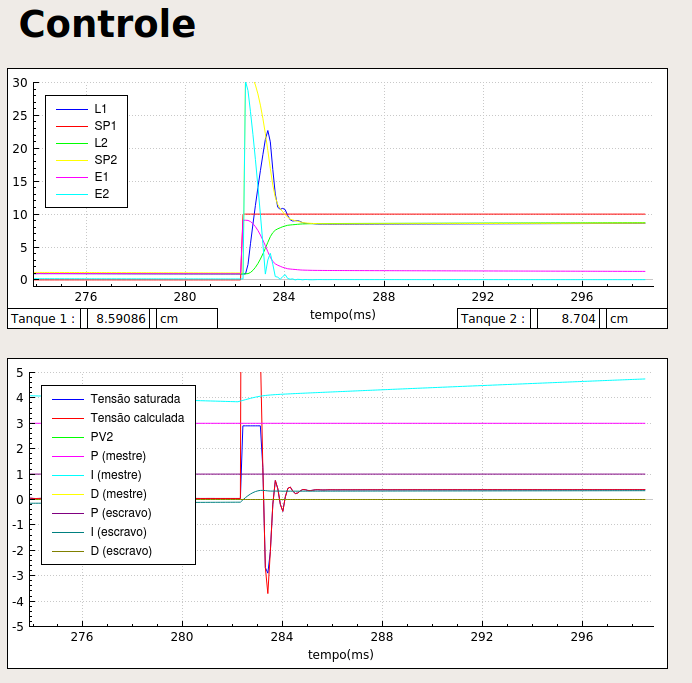
\includegraphics[width=11cm]{ImagensLab4/0.png}
\caption{Controle PI no mestre e no escravo com kp maior}
\label{img1}
\end{figure}

No terceiro teste, o kp do controlador 2 foi aumentado para 3. Esta mudança causou uma alta instabilidade no sistema, principalmente do tanque 1, cujo nível variou bastante entre 5 e 10 cm. A instabilidade causada pelo kp2 foi verificada novamente ao testar o sistema com dois PIs de variáveis kp=2, ki=0,05.
%[img9][img4]

\begin{figure}[H]
     \centering
     \subfloat[]{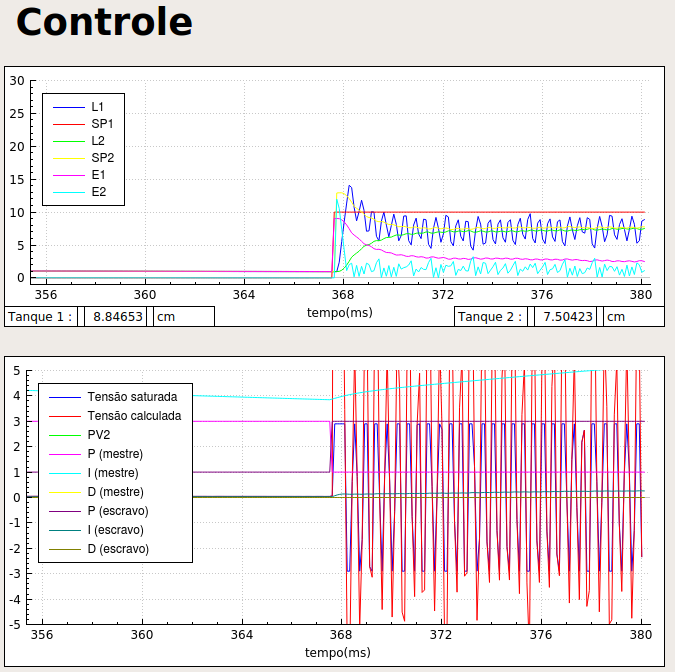
\includegraphics[width=7cm]{ImagensLab4/9.png}\label{img9}}    
\hspace{1cm}
     \subfloat[]{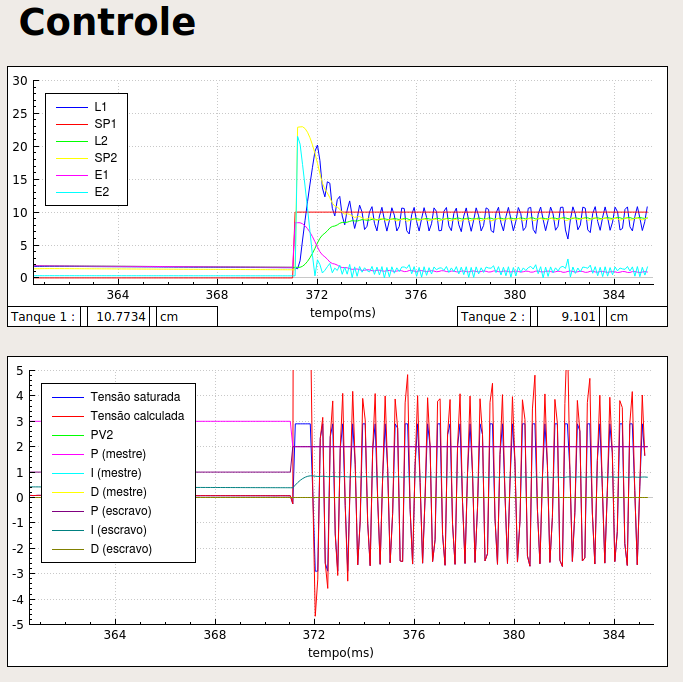
\includegraphics[width=7cm]{ImagensLab4/4.png}\label{img4}}
     
     \caption{Aumento do kp}
     \label{fig:ControlePI}
\end{figure}

Trocando o controlador 1 do segundo teste por um controlador PD (kp=3, kd=0,003), foi possível observar uma leve baixa do nível do tanque, com alterações pouco perceptíveis na fase transitória.
%[img10][img0]
\begin{figure}[H]
     \centering
     \subfloat[]{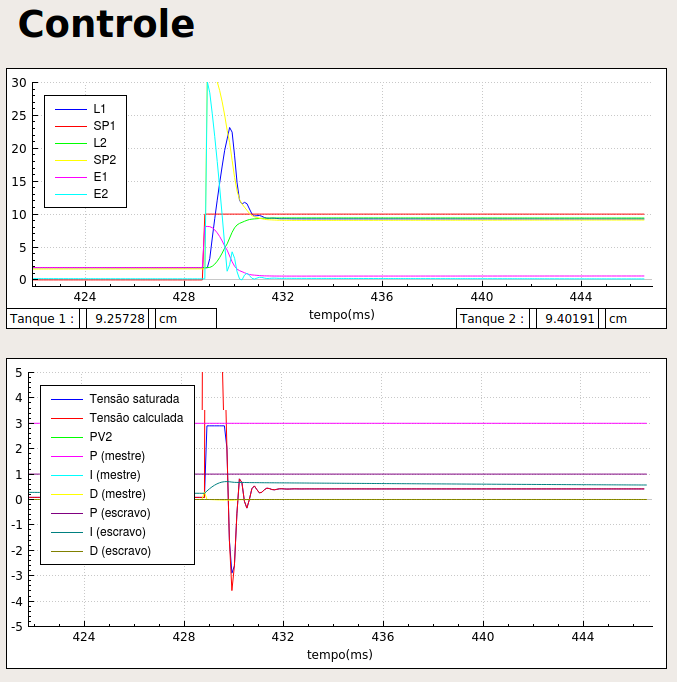
\includegraphics[width=7cm]{ImagensLab4/10.png}\label{img10}}    
\hspace{1cm}
     \subfloat[]{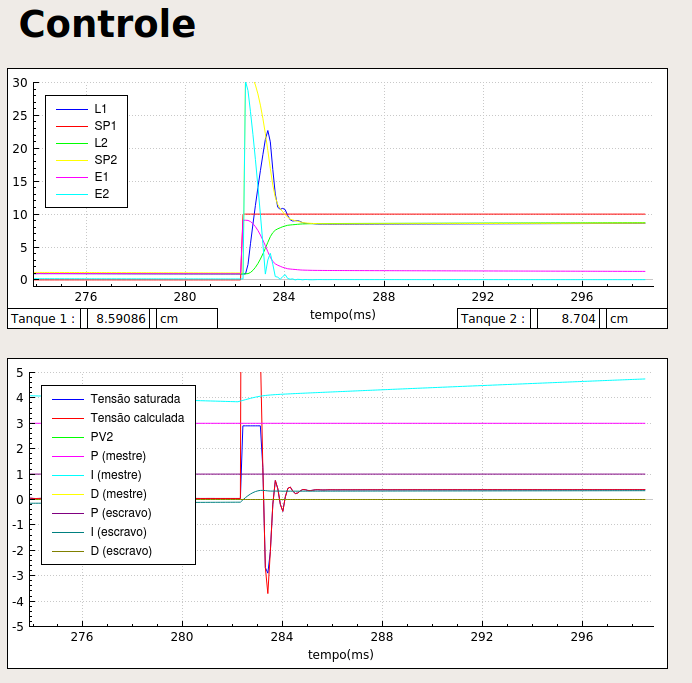
\includegraphics[width=7cm]{ImagensLab4/0.png}\label{img00}}
     
     \caption{Comparação entre Controle PD no escravo e PI no mestre e PI/PI}
     \label{fig:ControlePIPD}
\end{figure}

Em seguida, foi realizado um teste com uma dupla de controladores PID com kp=1, ki=0,01 e kd=0,001. Ao comparar com a dupla de PIs do primeiro teste, percebe-se um overshoot bem menor, com tempo de subida próximos e um nível mais baixo para a dupla de PIDs.
%[img5][img1]

\begin{figure}[H]
     \centering
     \subfloat[]{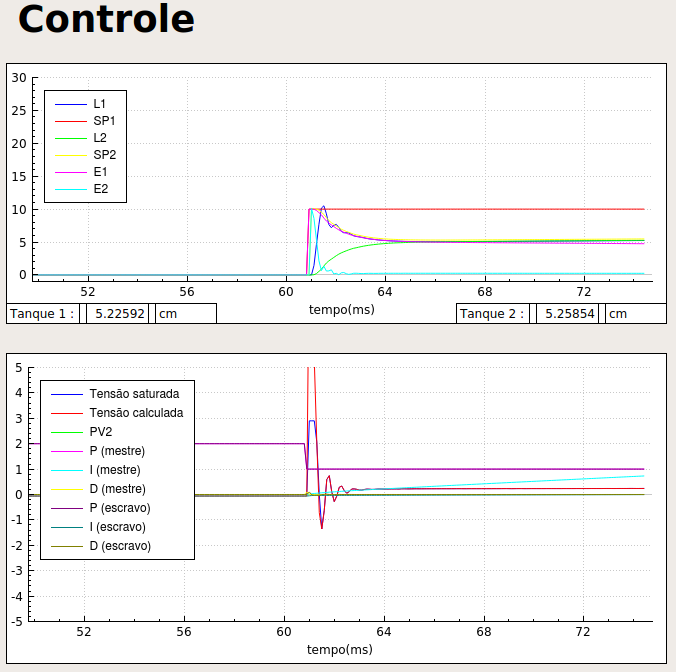
\includegraphics[width=7cm]{ImagensLab4/5.png}\label{img5}}    
\hspace{1cm}
     \subfloat[]{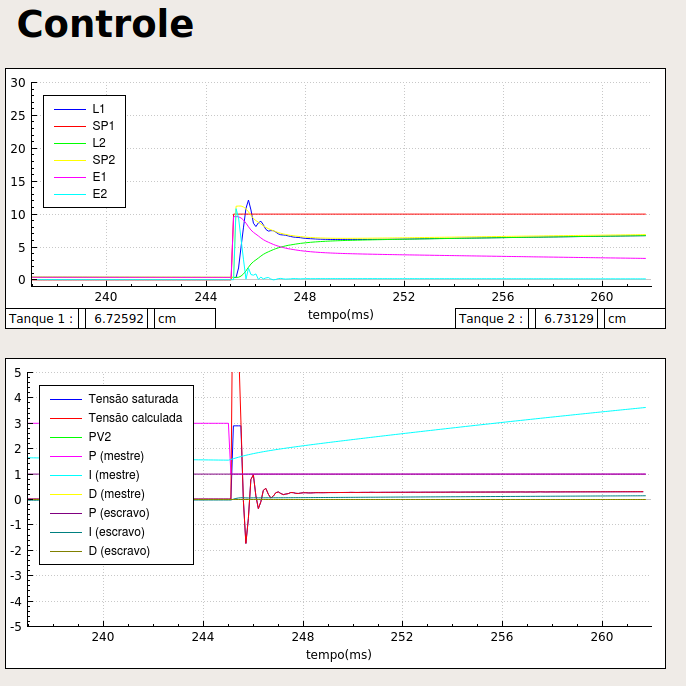
\includegraphics[width=7cm]{ImagensLab4/1.png}\label{img1}}
     
     \caption{Controle PID no escravo e PID no mestre}
     \label{fig:ControlePIDPID}
\end{figure}
Ao testar uma combinação P-PD, P com kp=3 e PD com kp=1 e kd=0,001, obtivemos um valor de nível bem mais próximo do desejado, com o sistema apresentando uma forma menos ondulatória do que nos testes anteriores. Ao trocar o PD por um PID, obtivemos uma fase transitória um pouco reduzida e uma queda considerável no nível do tanque.
%[img17][img8]

\begin{figure}[H]
     \centering
     \subfloat[]{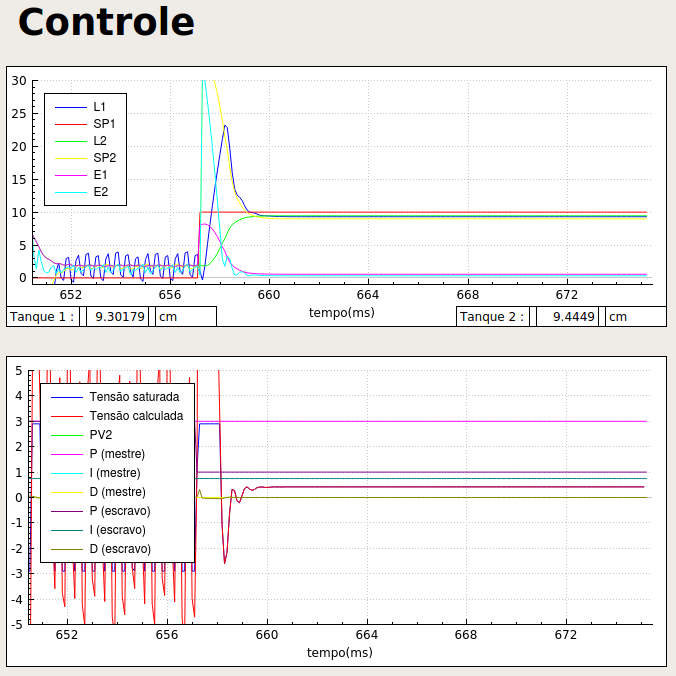
\includegraphics[width=7cm]{ImagensLab4/17.png}\label{img10}}    
\hspace{1cm}
     \subfloat[]{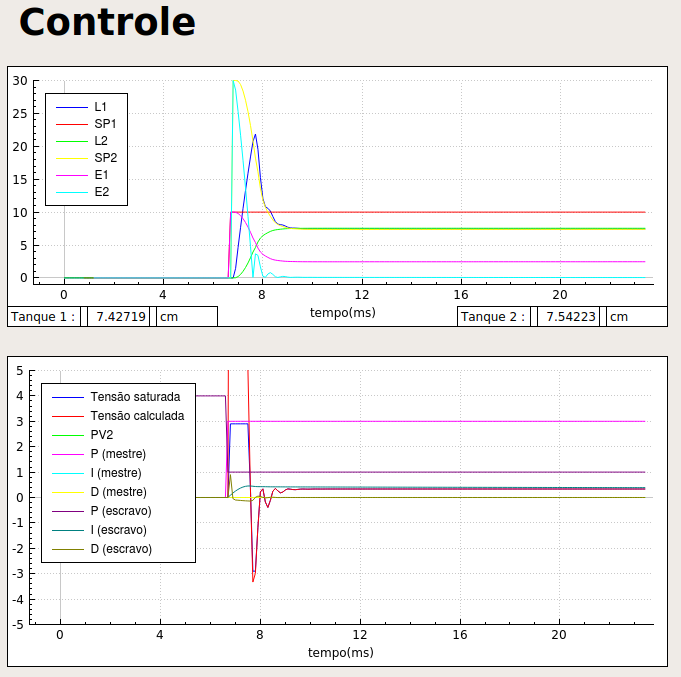
\includegraphics[width=7cm]{ImagensLab4/8.png}\label{img00}}
     
     \caption{Controle P no escravo e PD no mestre}
     \label{fig:ControleP-PD}
\end{figure}

Como último teste, foram realizadas combinações PI-PID, usando um PI similar ao controlador 1 do segundo teste e um PID com kp=1, ki=0,01 e kd=0,005, foram obtidos curvas menos ondulatórias que no segundo teste, com nível mais próximo do esperado e fase transitória de duração praticamente igual.
%[img3][img0]
\begin{figure}[H]
     \centering
     \subfloat[]{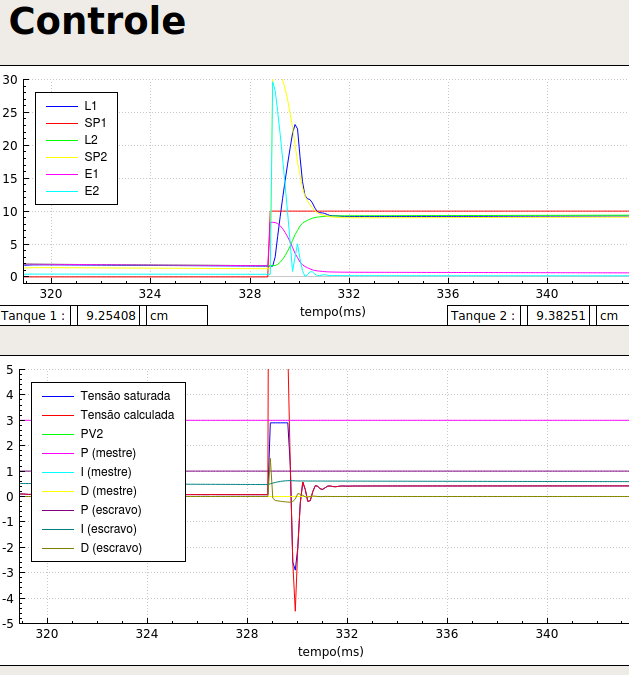
\includegraphics[width=7cm]{ImagensLab4/3.png}\label{img3}}    
\hspace{1cm}
     \subfloat[]{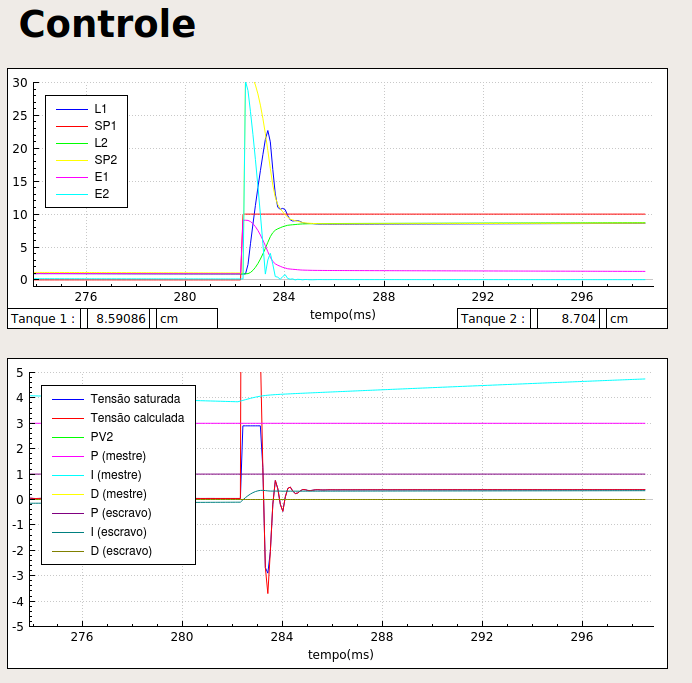
\includegraphics[width=7cm]{ImagensLab4/0.png}\label{img000}}
     
     \caption{Controle PI no escravo e PID no mestre}
     \label{fig:ControlePI}
\end{figure}

\hspace{4ex}Foram realizados posteriormente testes com propósito de comparar os resultados obtidos com um controlador de segunda ordem com os resultados obtidos com dois controladores. Inicialmente, com um controlador PID (kp = 1; ki = 0,05; kd = 0,005), foi obtido um sinal com um alto sobressinal (60,37\%), e tempos de acomodação e subida, respectivamente de 9,2 e 0,9 segundos. Ao adicionar um segundo controlador ao sistema, o sobressinal é praticamente eliminado. Foram utilizados como segundos controladores PI, PD e PID, para os três casos, os tempos de acomodação e subida ficaram, respectivamente, próximos a 90 e 60 segundos. 

%Imagens (2)

\begin{figure}[H]
     \centering
     \subfloat[]{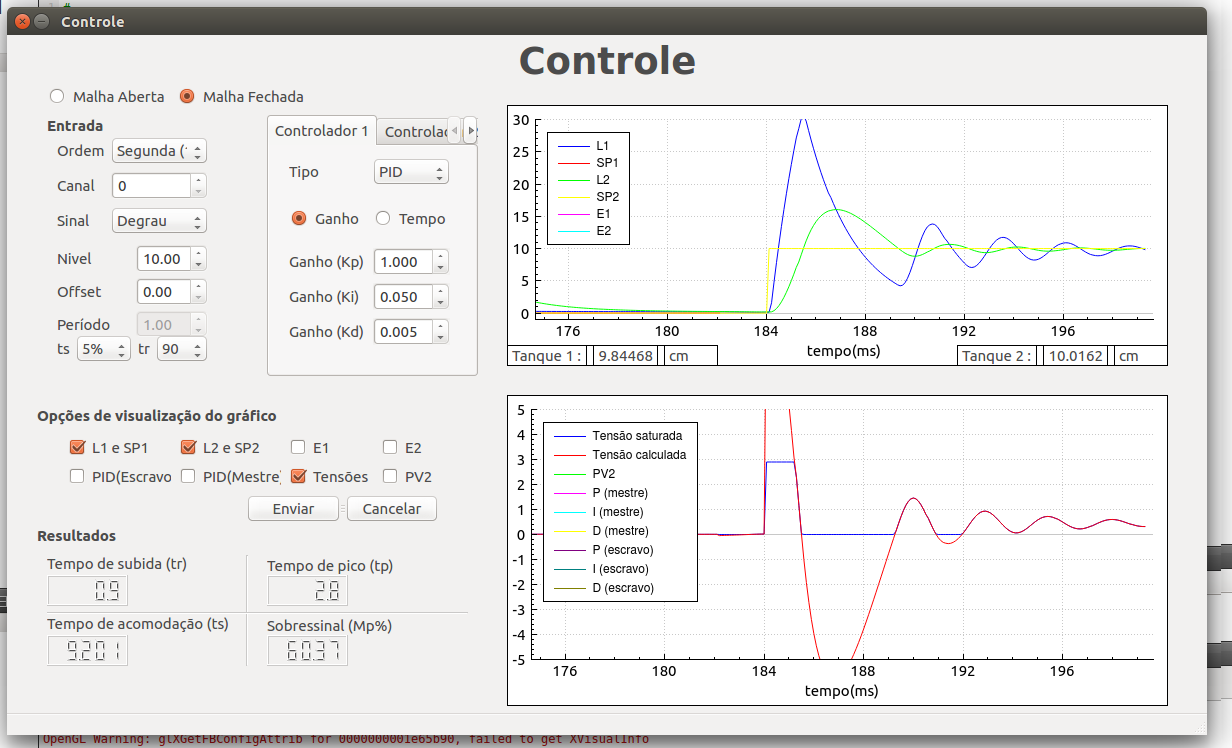
\includegraphics[width=11cm]{ImagensLab4/testes/2.png}\label{img2}}    
\hspace{1cm}
     \subfloat[]{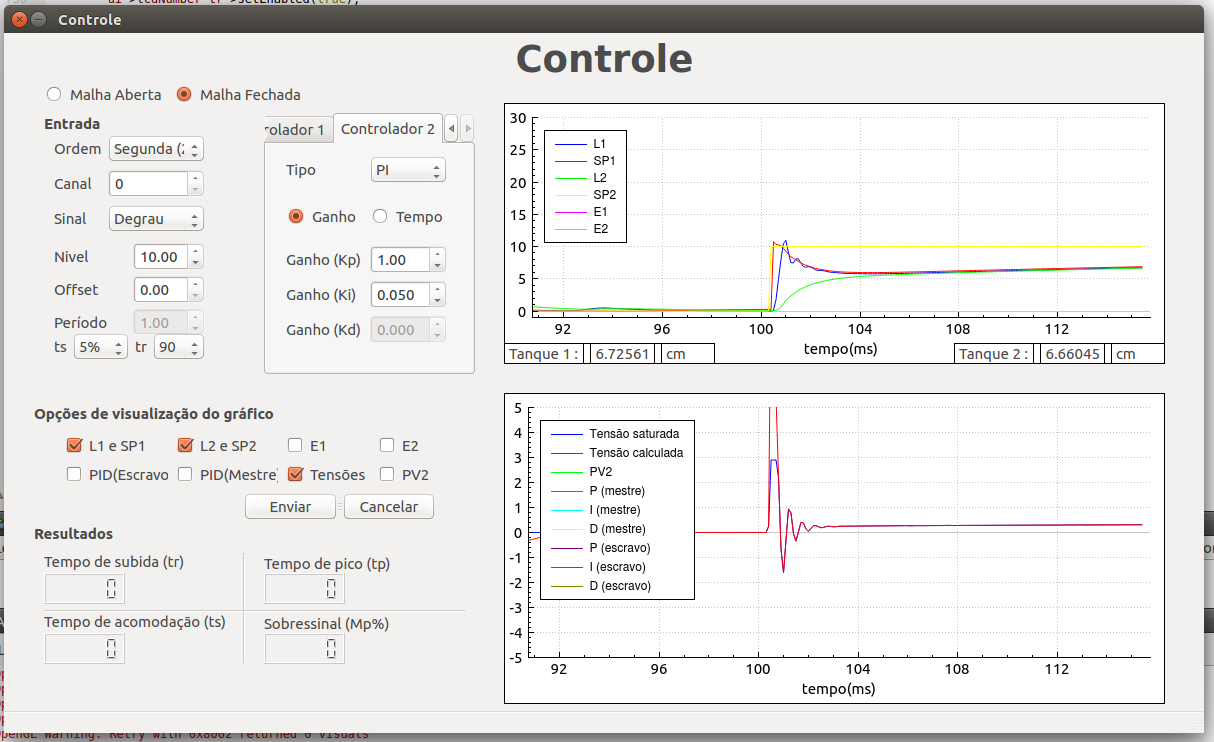
\includegraphics[width=7.4cm]{ImagensLab4/testes/2-1.png}\label{img2-1}}
\hspace{1cm}
     \subfloat[]{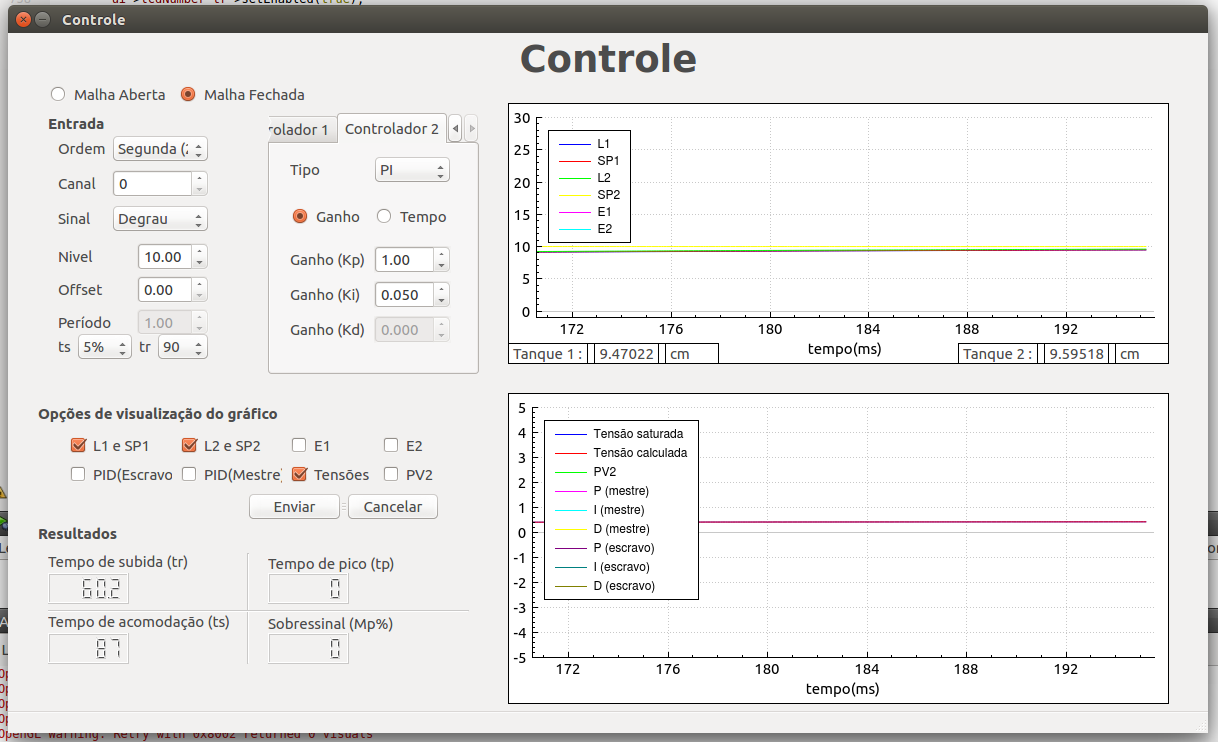
\includegraphics[width=7.4cm]{ImagensLab4/testes/2-1-1.png}\label{img2-1-1}}
\hspace{1cm}
     \subfloat[]{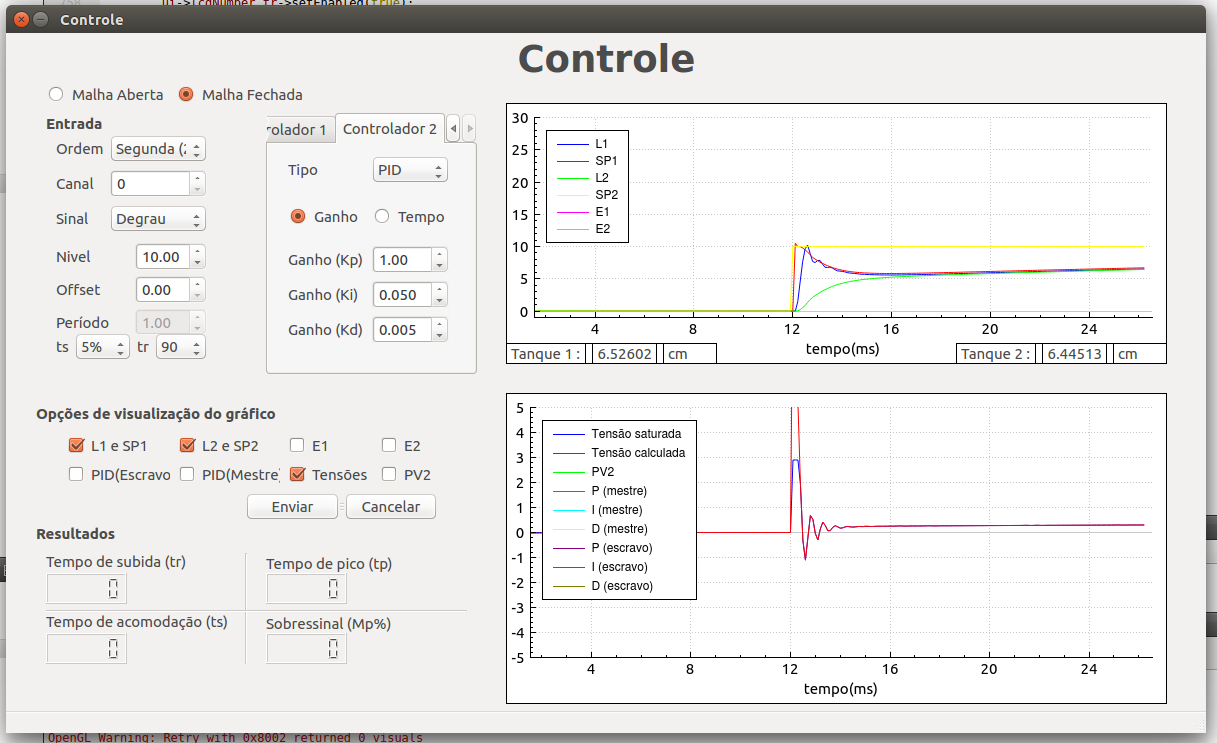
\includegraphics[width=7.4cm]{ImagensLab4/testes/2-2.png}\label{img2-2}}
\hspace{1cm}
     \subfloat[]{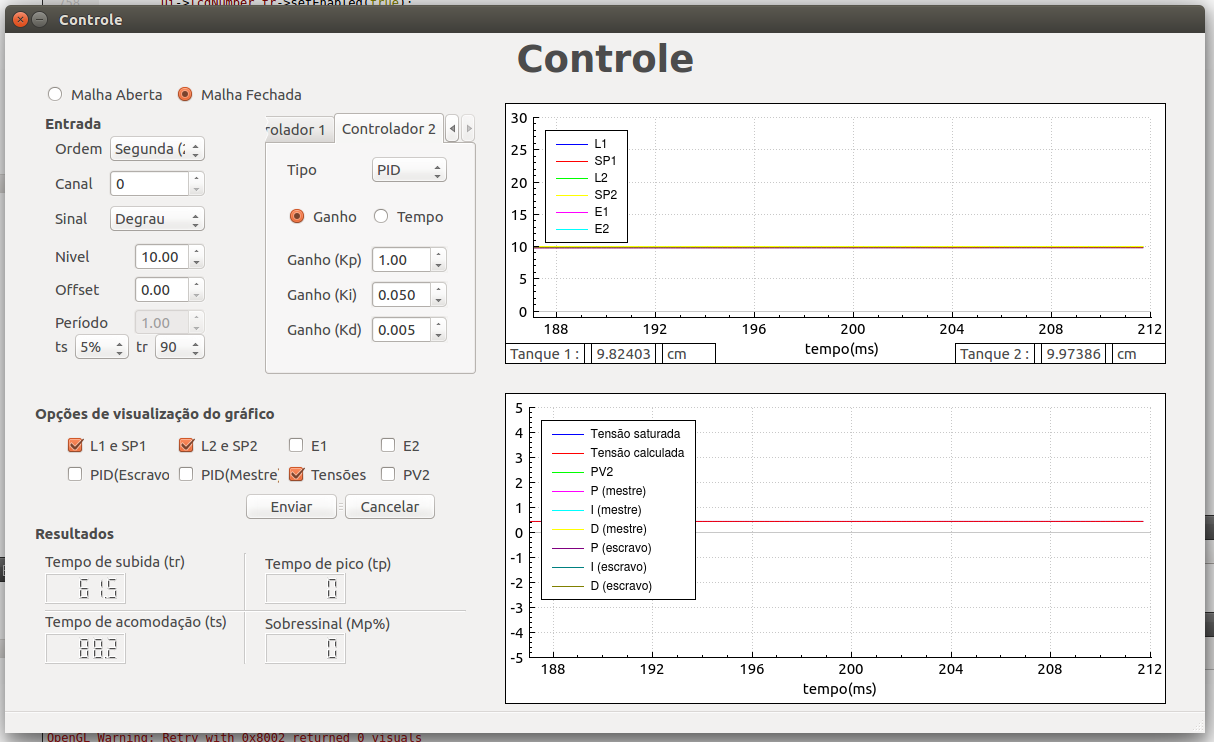
\includegraphics[width=7.4cm]{ImagensLab4/testes/2-2-1.png}\label{img2-2-1}}
\caption{Controle PID com kp=1, ki=0,05 e kd=0,005}
     \label{fig:ControlePID11}
\end{figure}
\begin{figure}[H]
     \centering
     \subfloat[]{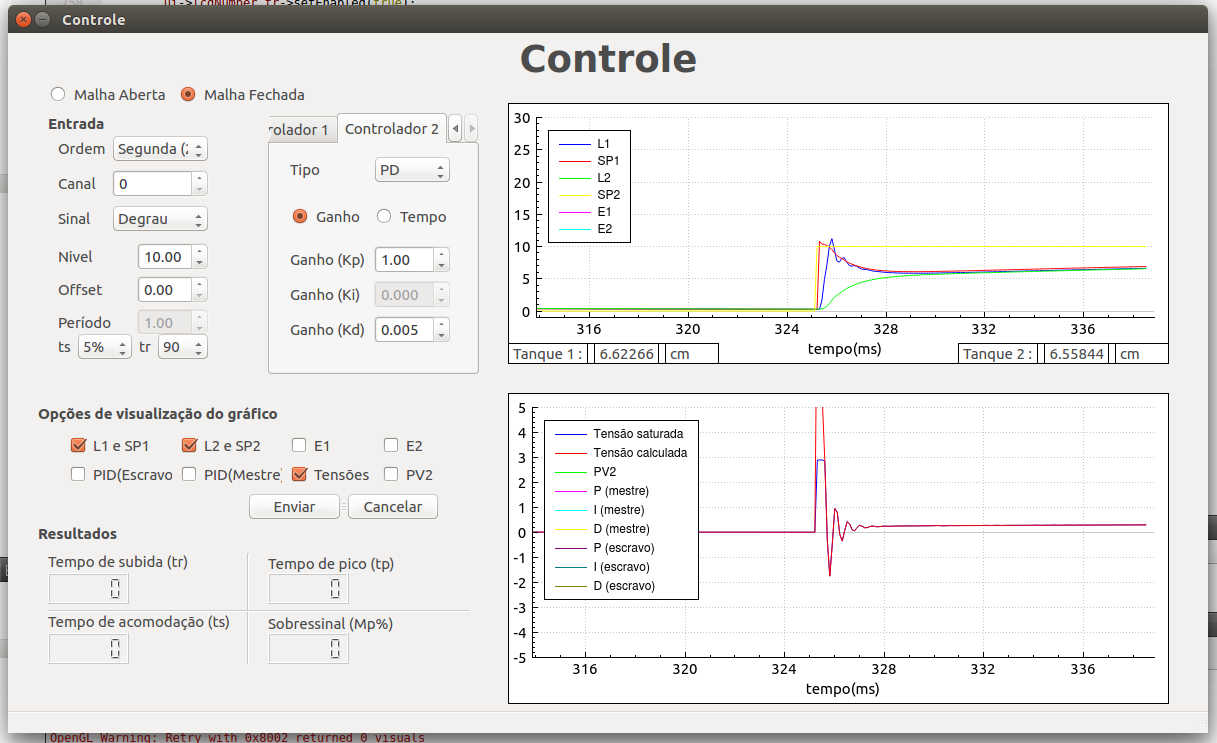
\includegraphics[width=7.4cm]{ImagensLab4/testes/2-3.png}\label{img2-3}}
\hspace{1cm}
     \subfloat[]{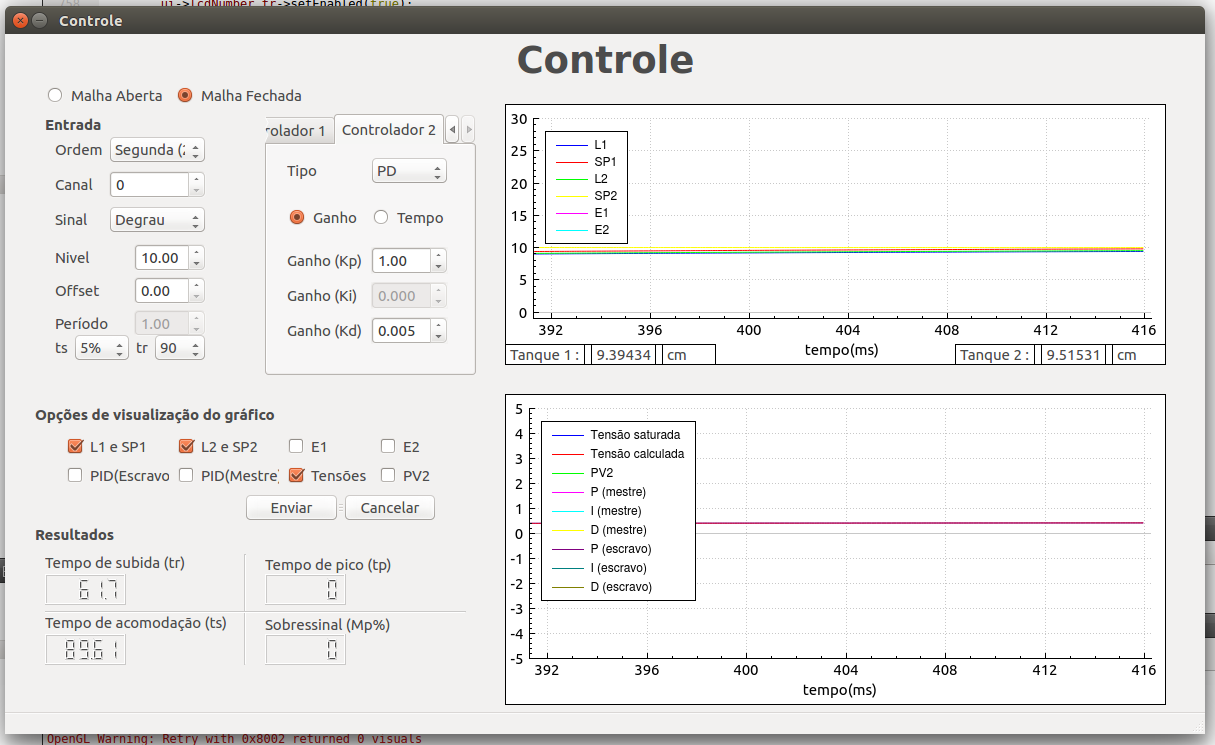
\includegraphics[width=7.4cm]{ImagensLab4/testes/2-3-1.png}\label{img2-3-1}}     
     \caption{Controle PID com kp=1, ki=0,05 e kd=0,005}
     \label{fig:ControlePID12}
\end{figure}


Foi feito para um controlador PI (kp=1; ki=0,05) o mesmo que o feito com o controlador PID, unindo-o a três controladores diferentes PI, PD e PID - um por vez. O resultado obtido foi parecido com o do teste anterior, com o alto sobressinal do PI (58,91\%) sendo eliminado, e os tempos de subida e acomodação sofrendo grande aumento. Neste exemplo, a diferença nos tempos de subida e acomodação foi um pouco mais visível, com a combinação PI-PI sendo mais rápida que a PI-PID em aproximadamente 3 segundos para tr (tempo de subida) e 4 segundos para ts (tempo de acomodação). A combinação PI-PID por sua vez foi mais rápida que a PI-PD aproximadamente pela mesma diferença – 3s para tr e 4s para ts.
\\
%Imagens (3)


\begin{figure}[H]
     \centering
     \subfloat[]{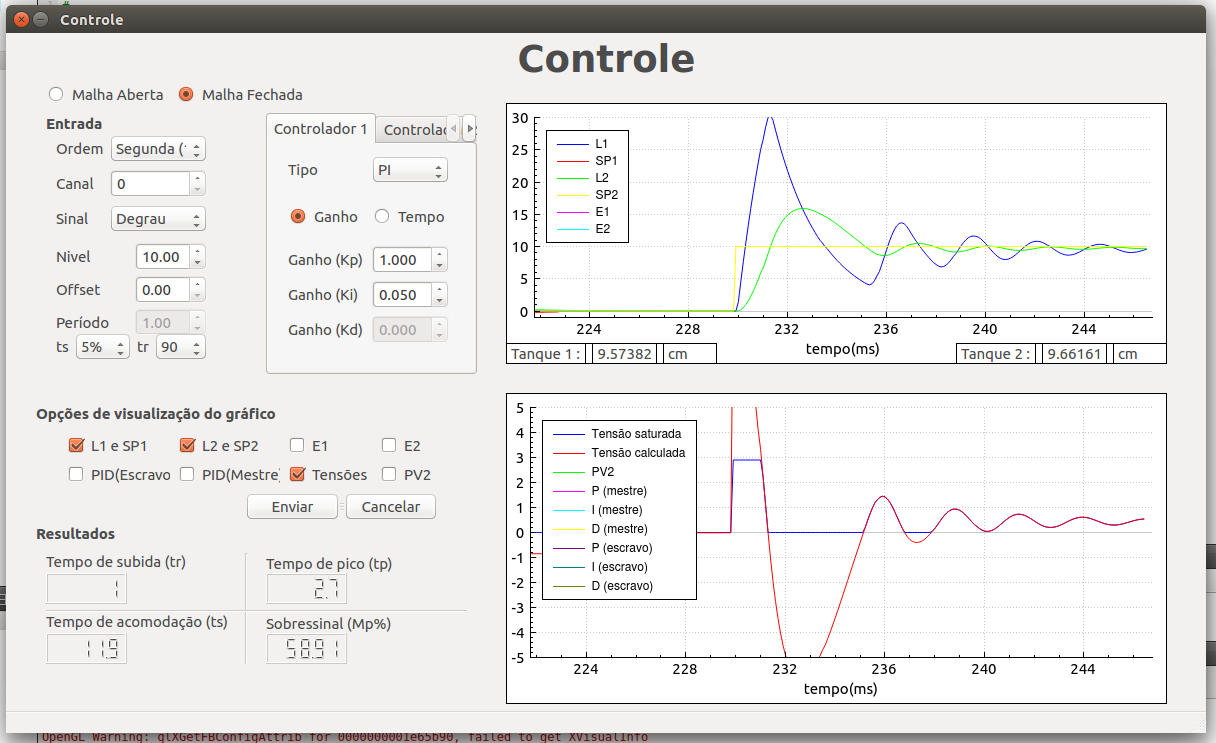
\includegraphics[width=11cm]{ImagensLab4/testes/3.png}\label{img3}}    
\caption{Controle PI com kp=1 e ki=0,05}
     \label{fig:ControlePI}
\end{figure}
\begin{figure}[H]
     \centering
     \subfloat[]{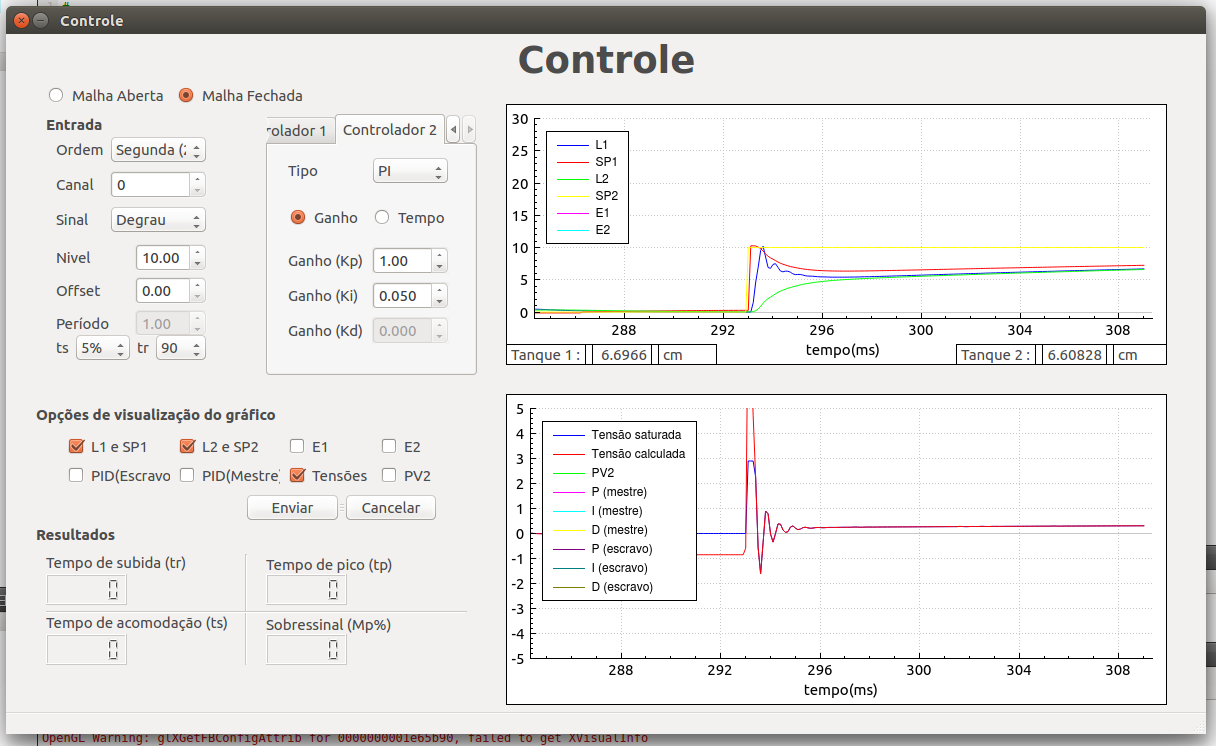
\includegraphics[width=7.4cm]{ImagensLab4/testes/3-2.png}\label{img3-1}}
\hspace{1cm}
     \subfloat[]{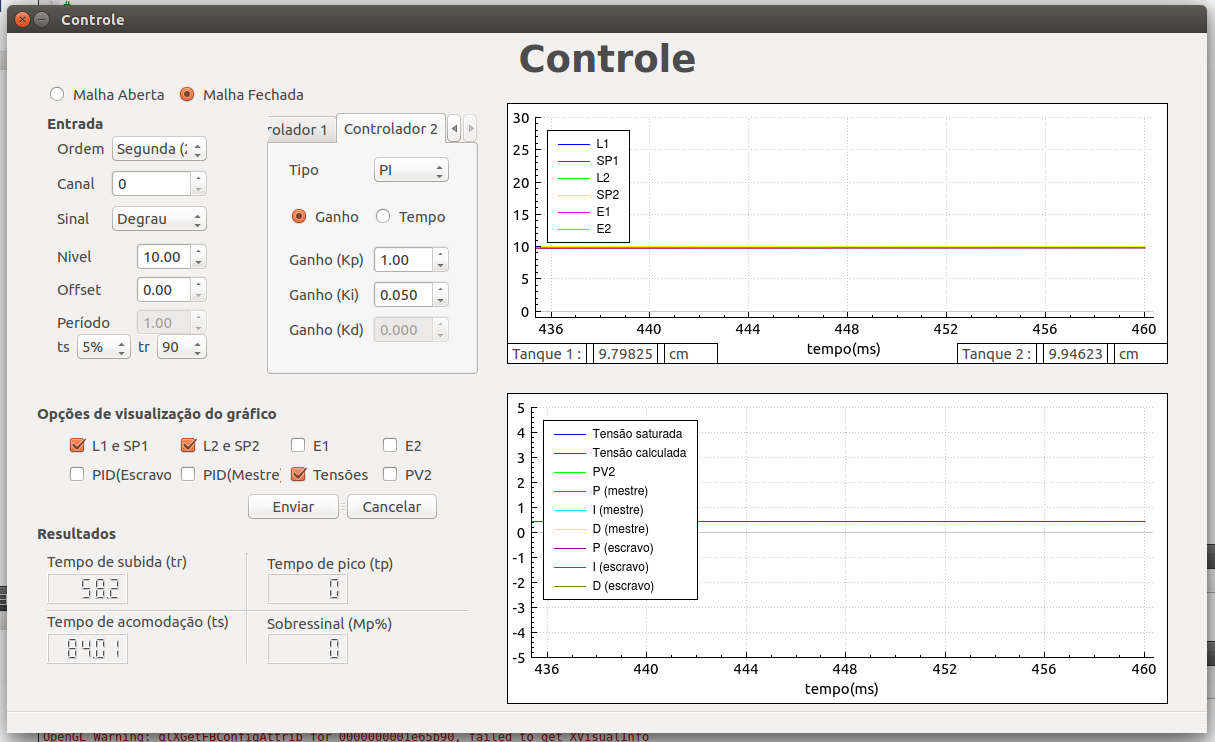
\includegraphics[width=7.4cm]{ImagensLab4/testes/3-2-1.png}\label{img3-1-1}}
\hspace{1cm}
     \subfloat[]{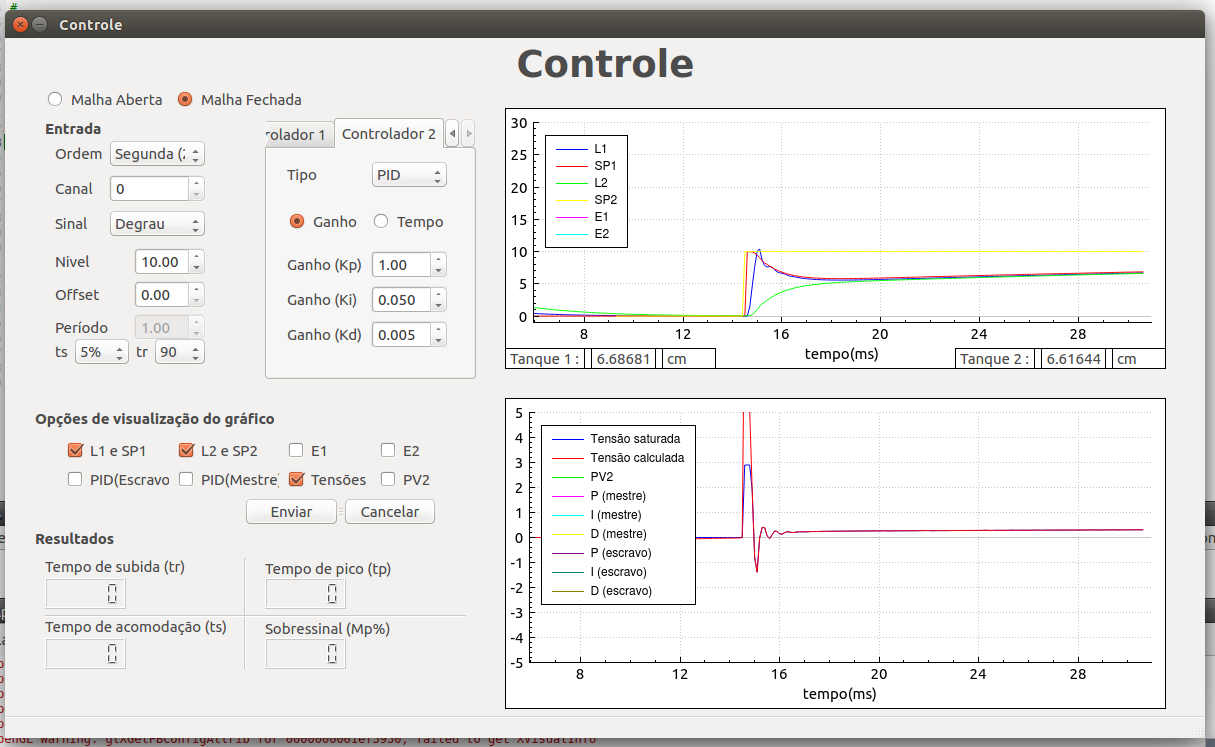
\includegraphics[width=7.4cm]{ImagensLab4/testes/3-3.png}\label{img3-2}}
\hspace{1cm}
     \subfloat[]{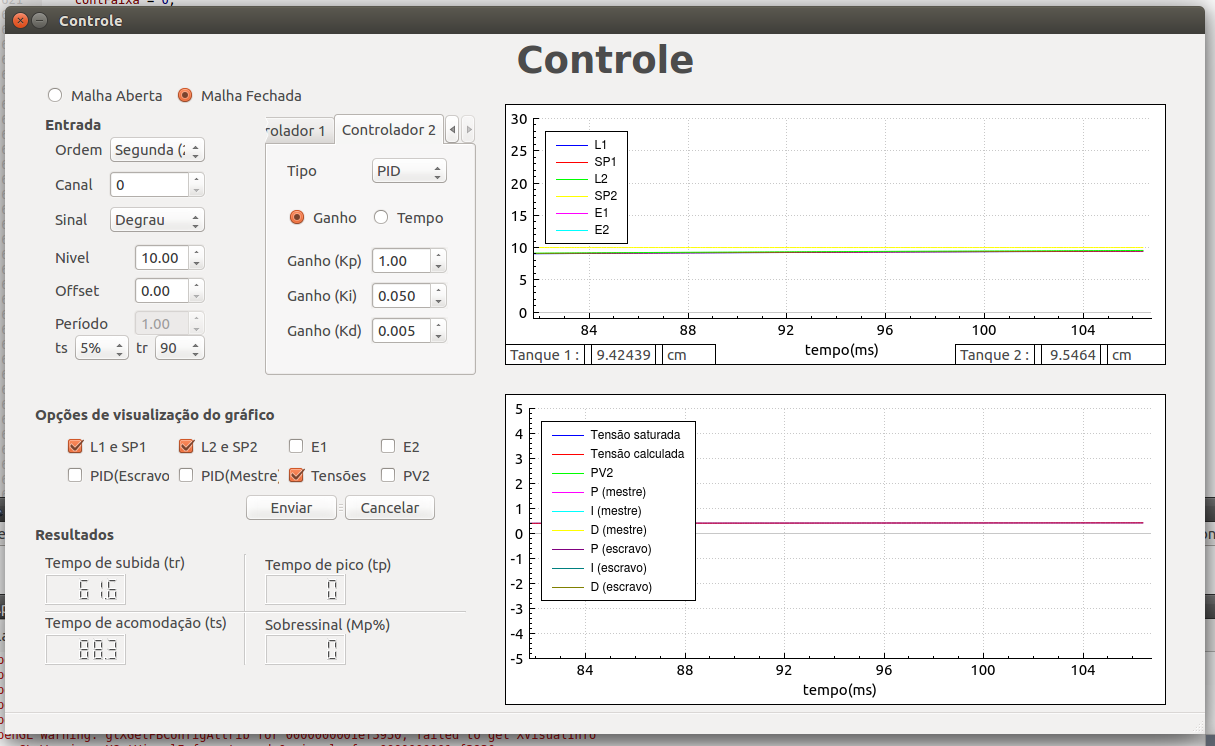
\includegraphics[width=7.4cm]{ImagensLab4/testes/3-3-1.png}\label{img3-2-1}}
\hspace{1cm}
     \subfloat[]{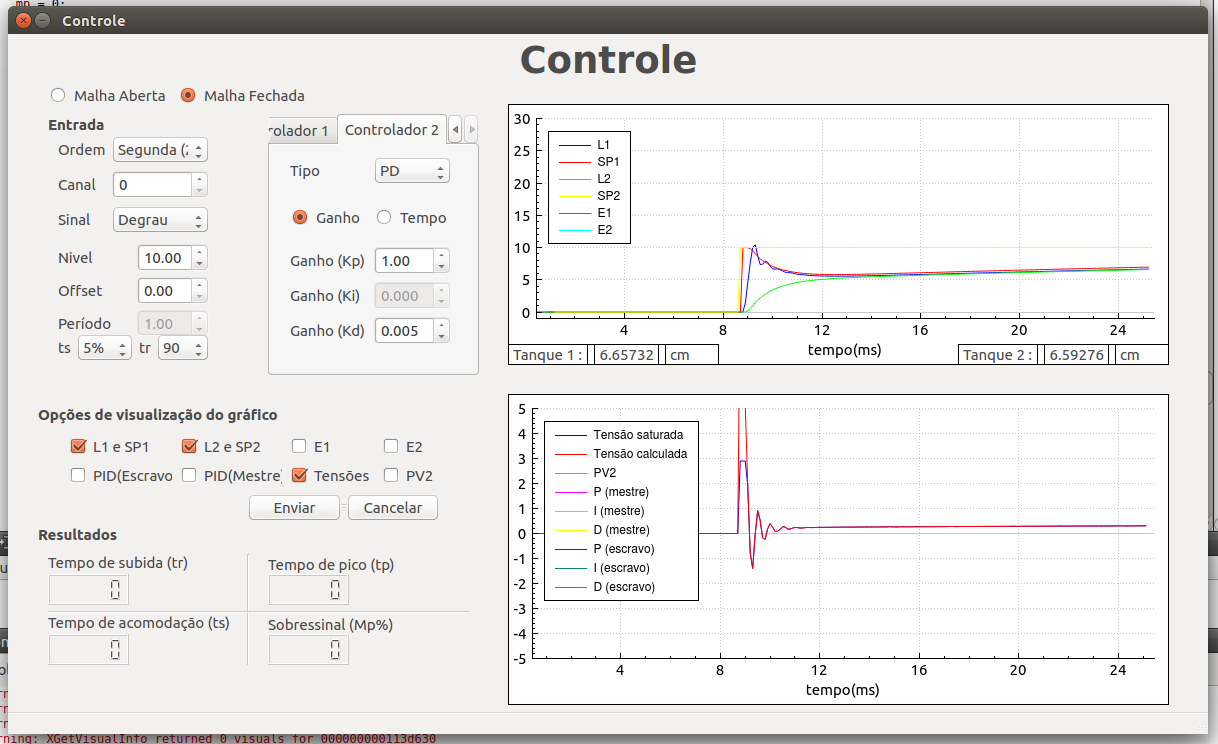
\includegraphics[width=7.4cm]{ImagensLab4/testes/3-4.png}\label{img3-3}}
\hspace{1cm}
     \subfloat[]{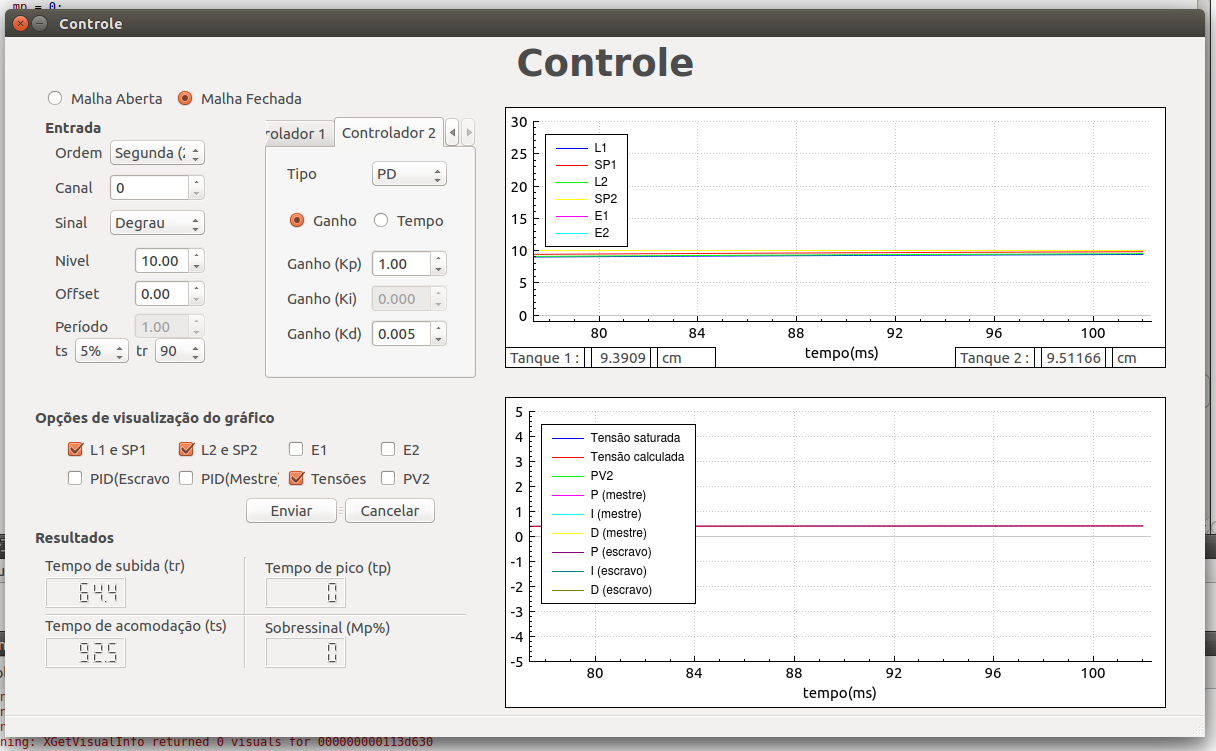
\includegraphics[width=8cm]{ImagensLab4/testes/3-4-1.png}\label{img3-3-1}}     
     \caption{Controle PI com kp=1 e ki=0,05}
     \label{fig:ControlePI}
\end{figure}



No terceiro teste foi usado um PID com kp duas vezes maior que o do primeiro teste, obtendo um sistema de um controlador menos estável. Quando aplicados controladores secundários semelhantes aqueles dos testes anteriores, é possível perceber um maior nível do tanque no curto prazo, com o mesmo chegando a atingir 17cm após 1s. Porém, se por um lado, o nível dos tanques está maior nos primeiros 5s, a velocidade de subida de nível é menor que em kp=1, fazendo com que o tempo de acomodação suba em todos os casos. O tempo de subida também foi alterado, apresentando inclusive uma redução para o caso PID-PID, mas também apresentando aumento para PI e para PD.

%Imagens (4) – menos 4-2


\begin{figure}[H]
     \centering
     \subfloat[]{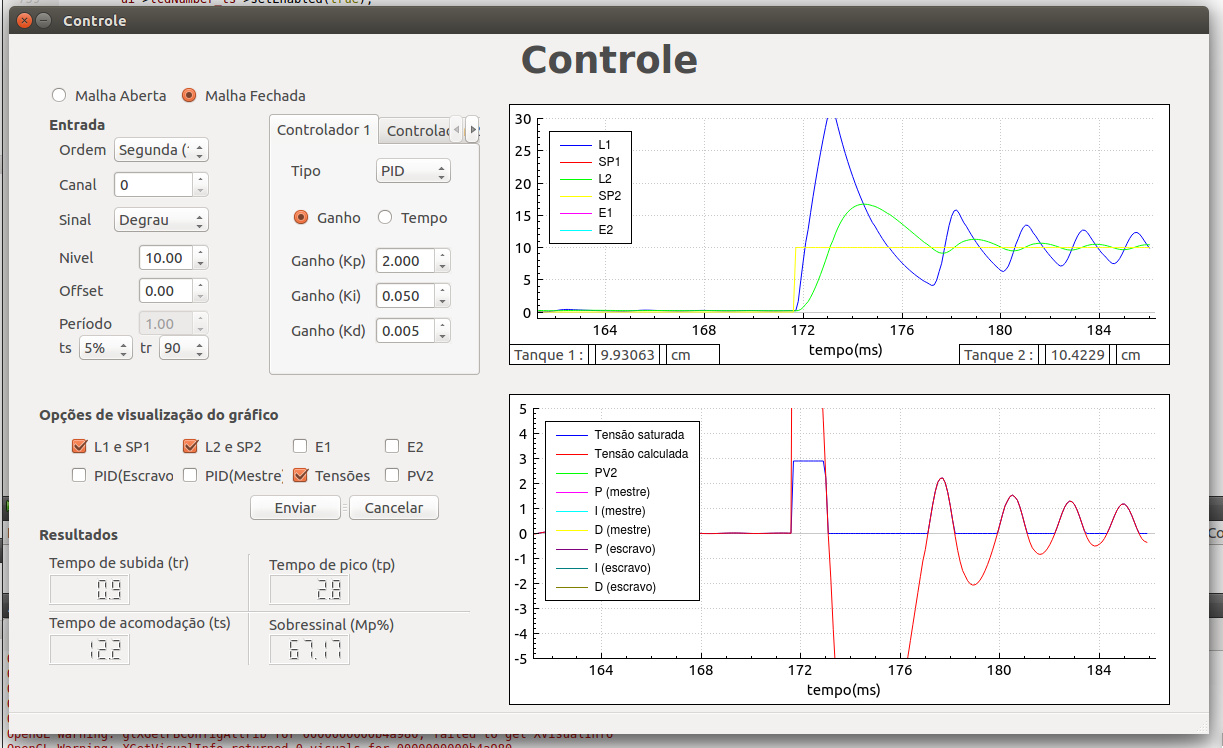
\includegraphics[width=11cm]{ImagensLab4/testes/4.png}\label{img4}}    
\hspace{1cm}
     \subfloat[]{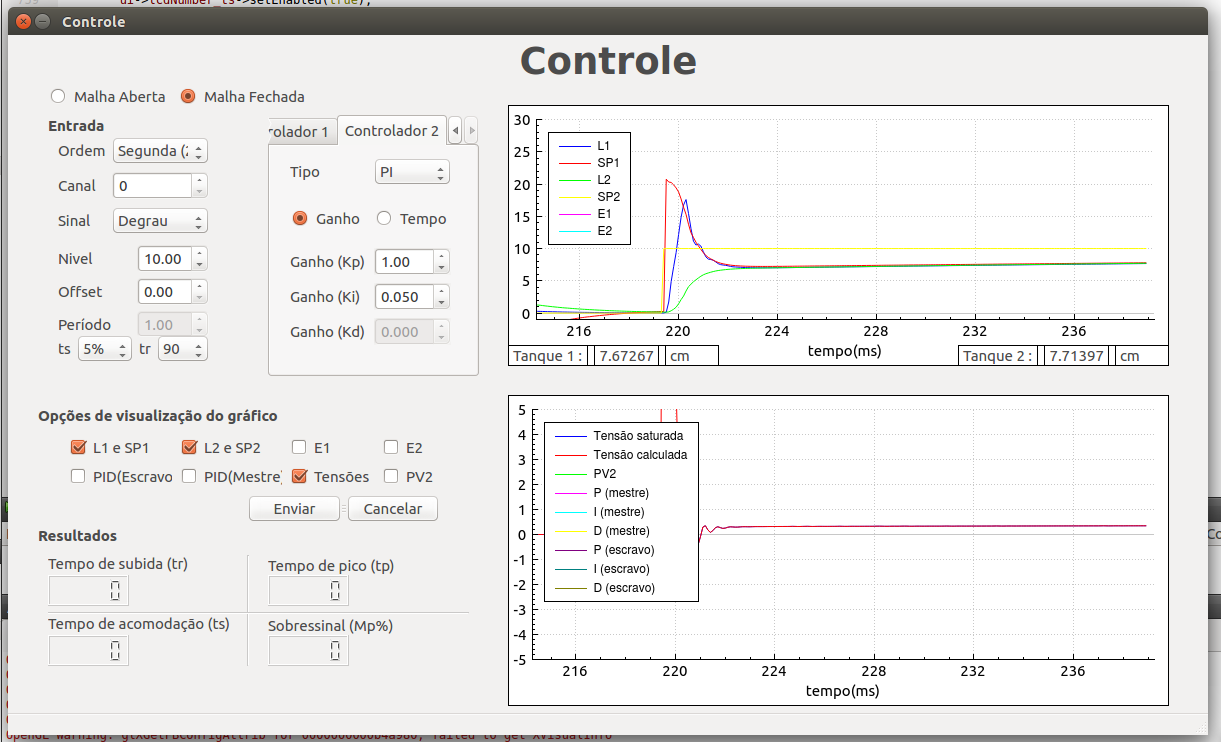
\includegraphics[width=7.4cm]{ImagensLab4/testes/4-1.png}\label{img4-1}}
\hspace{1cm}
     \subfloat[]{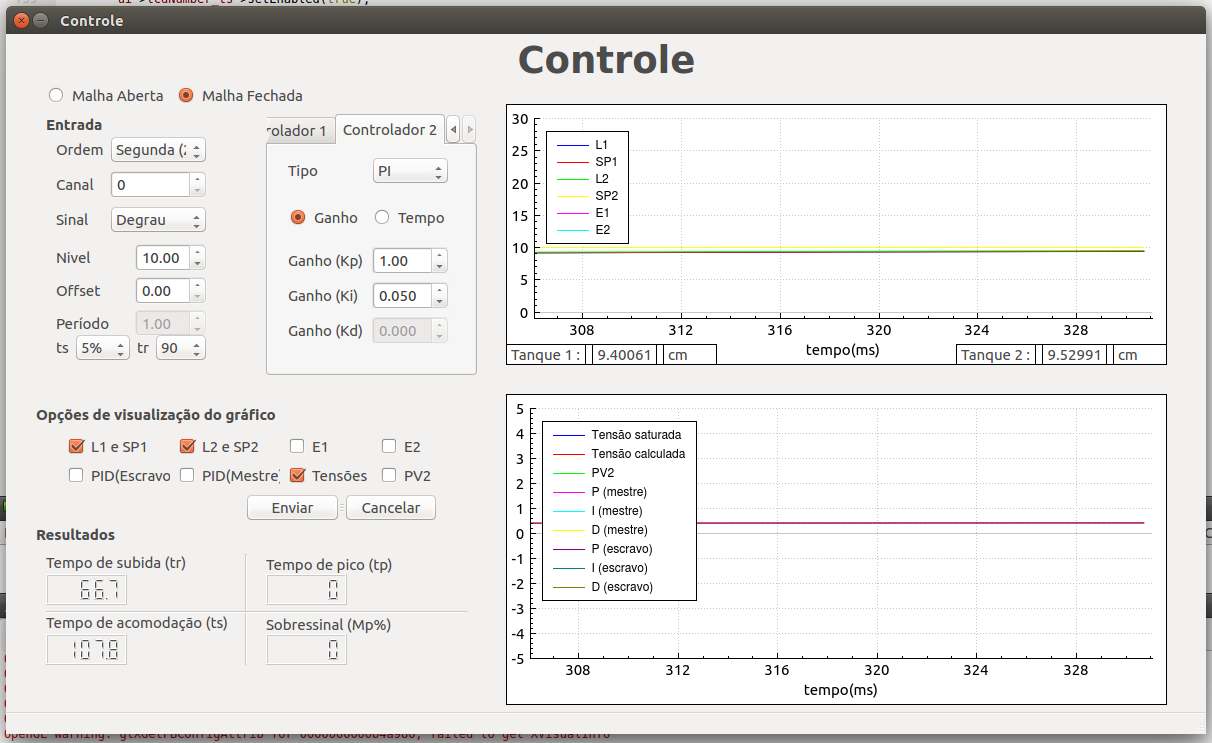
\includegraphics[width=7.4cm]{ImagensLab4/testes/4-1-1.png}\label{img4-1-1}}
\hspace{1cm}
     \subfloat[]{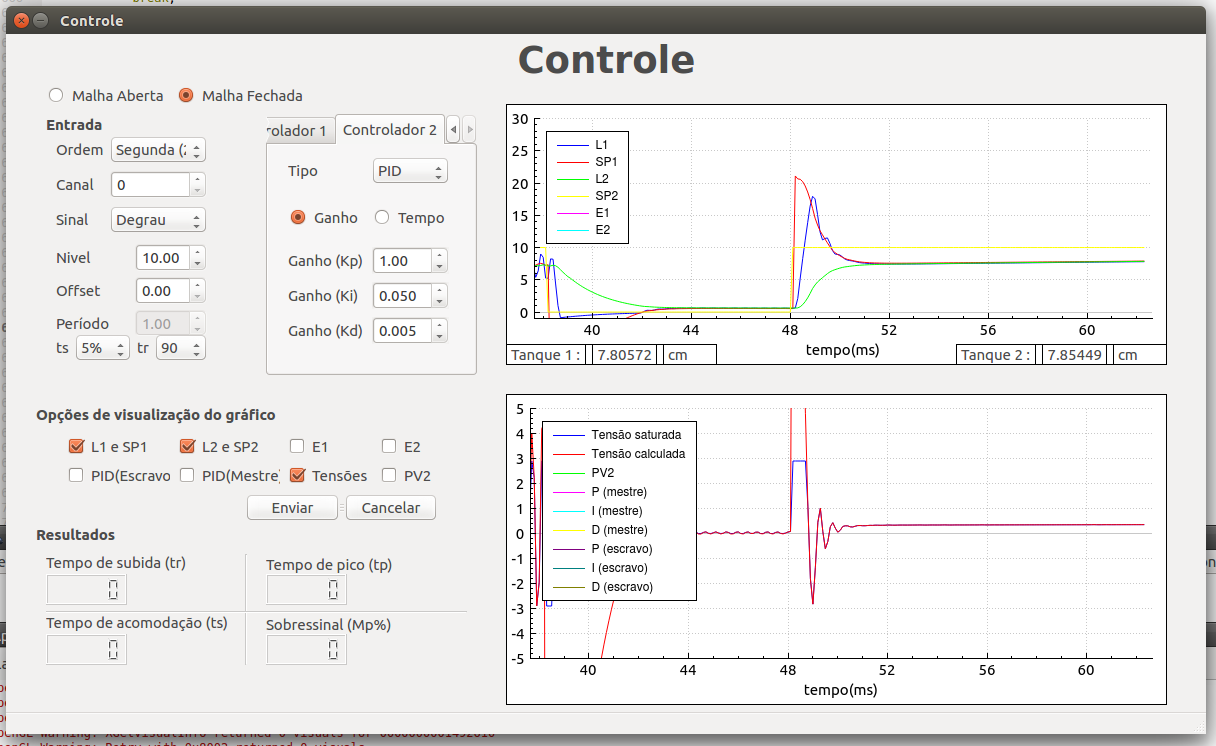
\includegraphics[width=7.4cm]{ImagensLab4/testes/4-3.png}\label{img4-2}}
\hspace{1cm}
     \subfloat[]{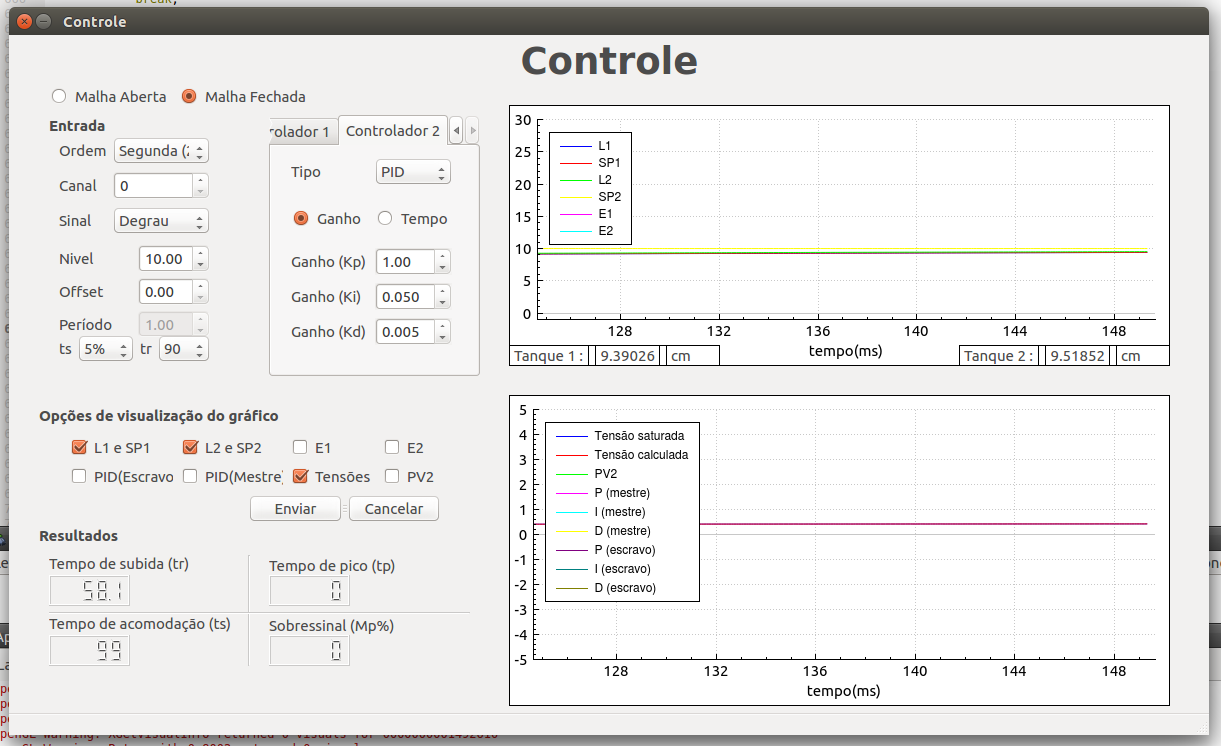
\includegraphics[width=7.4cm]{ImagensLab4/testes/4-3-1.png}\label{img4-2-1}}
\hspace{1cm}
     \subfloat[]{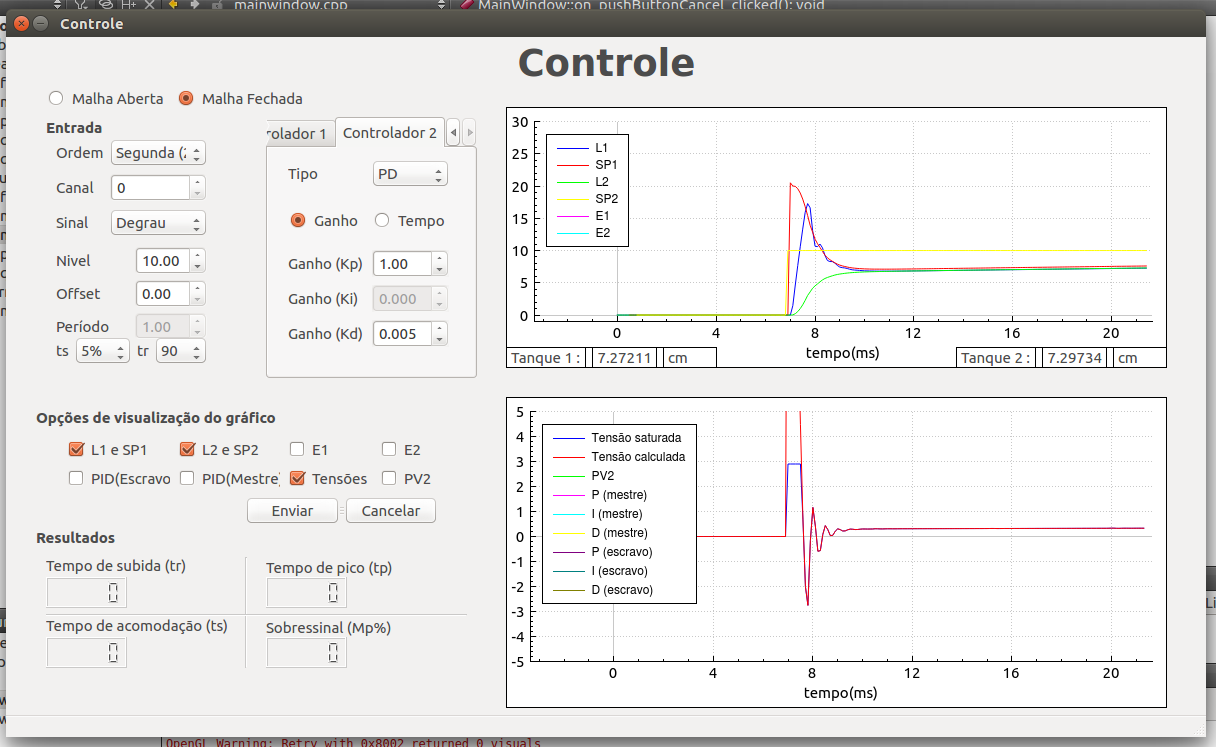
\includegraphics[width=7.4cm]{ImagensLab4/testes/4-4.png}\label{img4-3}}
\hspace{1cm}
     \subfloat[]{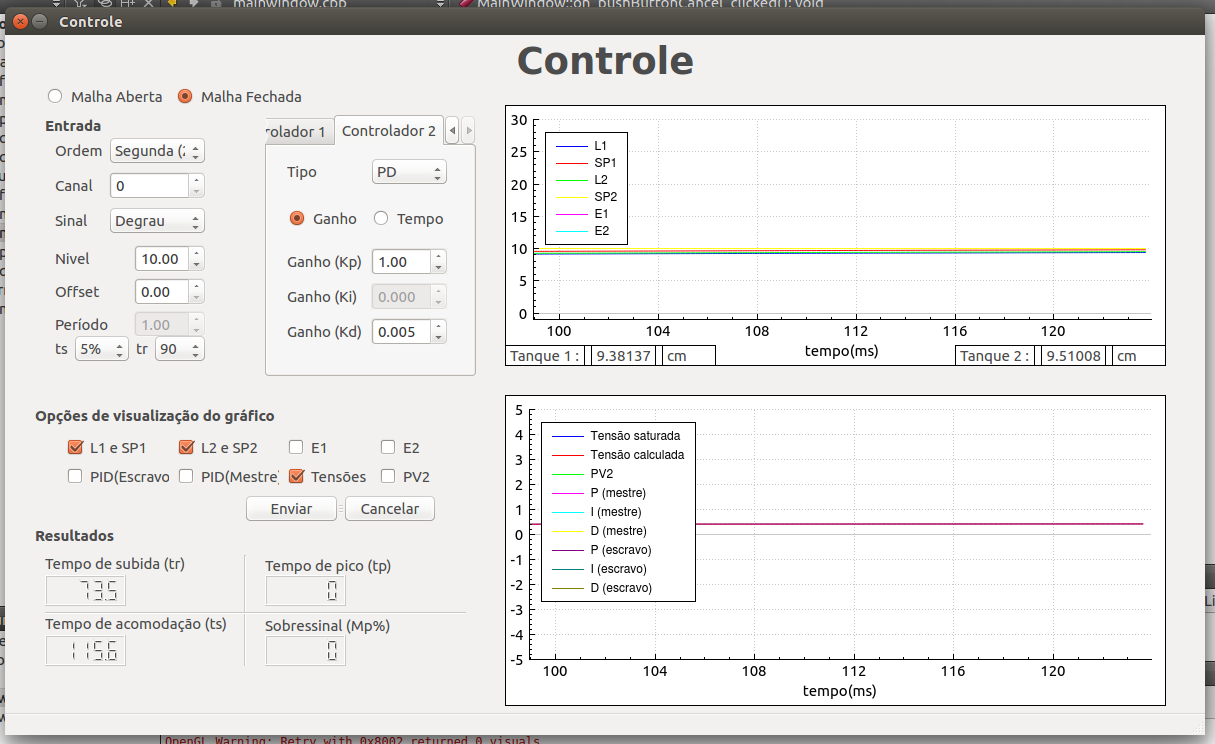
\includegraphics[width=7.4cm]{ImagensLab4/testes/4-4-1.png}\label{img4-3-1}}     
     \caption{PID com kp=2,  ki=0,05 e kd=0,005}
     \label{fig:ControlePID2}
\end{figure}

\newpage
Um pequeno teste para C2 com kp=2 mostrou uma grande instabilidade do sistema para o aumento de kp no controlador secundário.
\hspace{1cm}
%Imagem 4-2

\begin{figure}[!h]
\centering
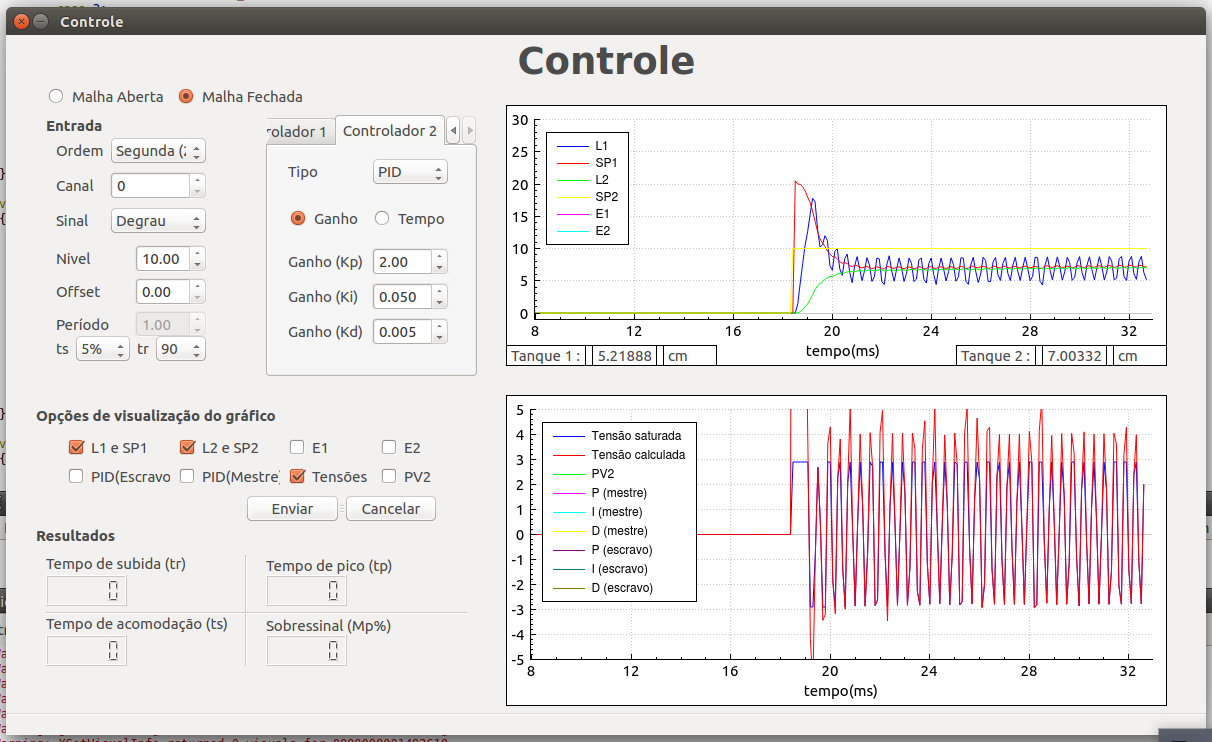
\includegraphics[width=11cm]{ImagensLab4/testes/4-2.png}
\caption{PID escravo com kp=2}
\label{img4-4}
\end{figure}

Como teste final, foram feitas alterações em ki e kd em um controlador primário PID de kp=2. O controlador secundário foi para todos os casos um PI com kp=1 e ki=0,05. As alterações em ki alteraram largamente os tempos de subida e acomodação, se para ki=0,05, no teste passado, foi obtido ts = 107,8s, para ki=0,03 tivemos ts = 186,2s – 72,7\% de aumento – e para ki=0,01 tivemos ts = 560,9s – 420,3\% de aumento em relação a ki=0,05 – com os tempos de subida seguindo percentuais de aumento próximos. A alteração de kd, de 0,005 para 0,001 teve efeito menor nos tempos ts e tr, com aumento de pouco mais de 3 segundos para ambos.

%Imagens (5)


\begin{figure}[H]
     \centering
     \subfloat[]{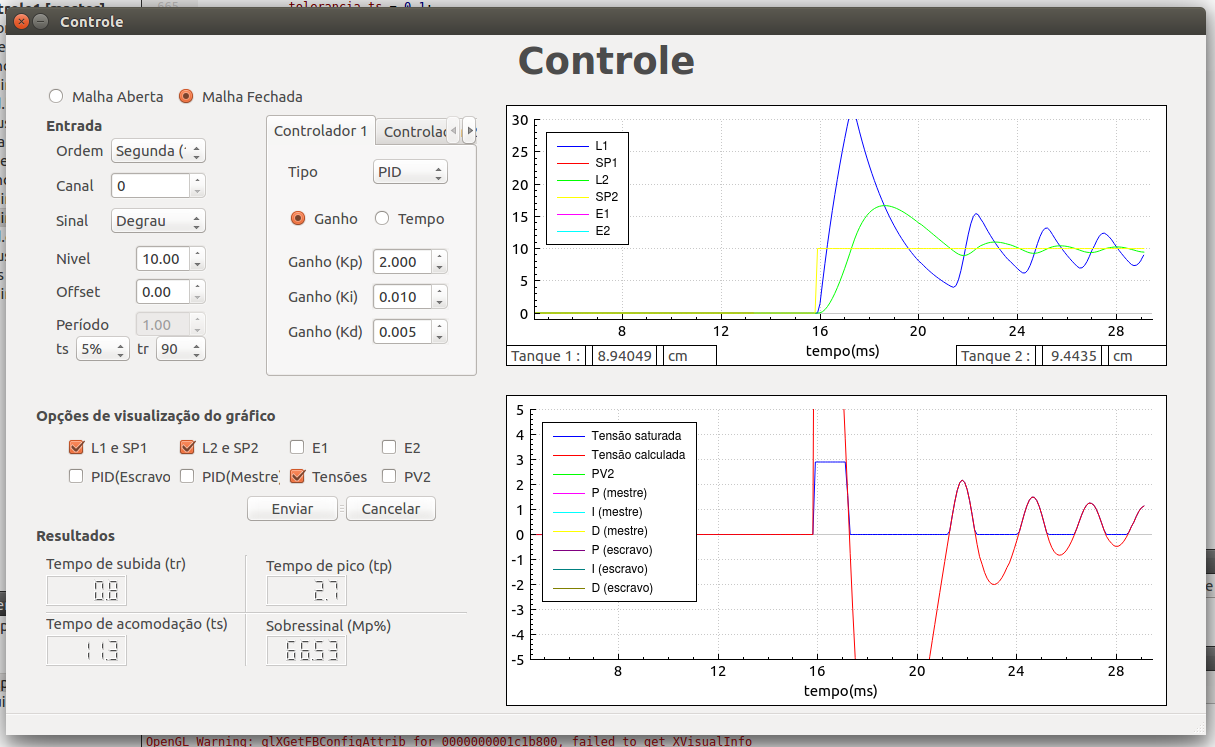
\includegraphics[width=11cm]{ImagensLab4/testes/5.png}\label{img5}}    
\caption{Controle PID com kp=2 e valores variáveis para ki e kd}
     \label{fig:ControlePID2 com variação de ki e kd}
\end{figure}
\begin{figure}[H]
     \centering
     \subfloat[]{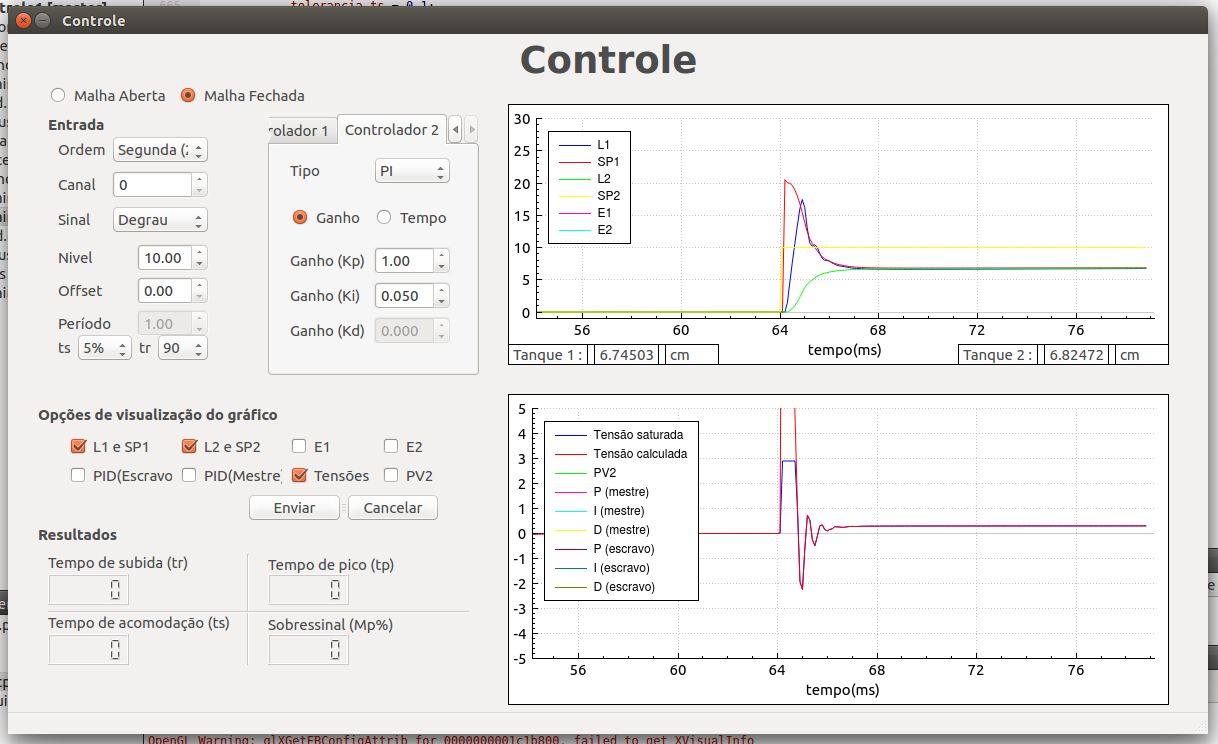
\includegraphics[width=7.4cm]{ImagensLab4/testes/5-1.png}\label{img5-1}}
\hspace{1cm}
     \subfloat[]{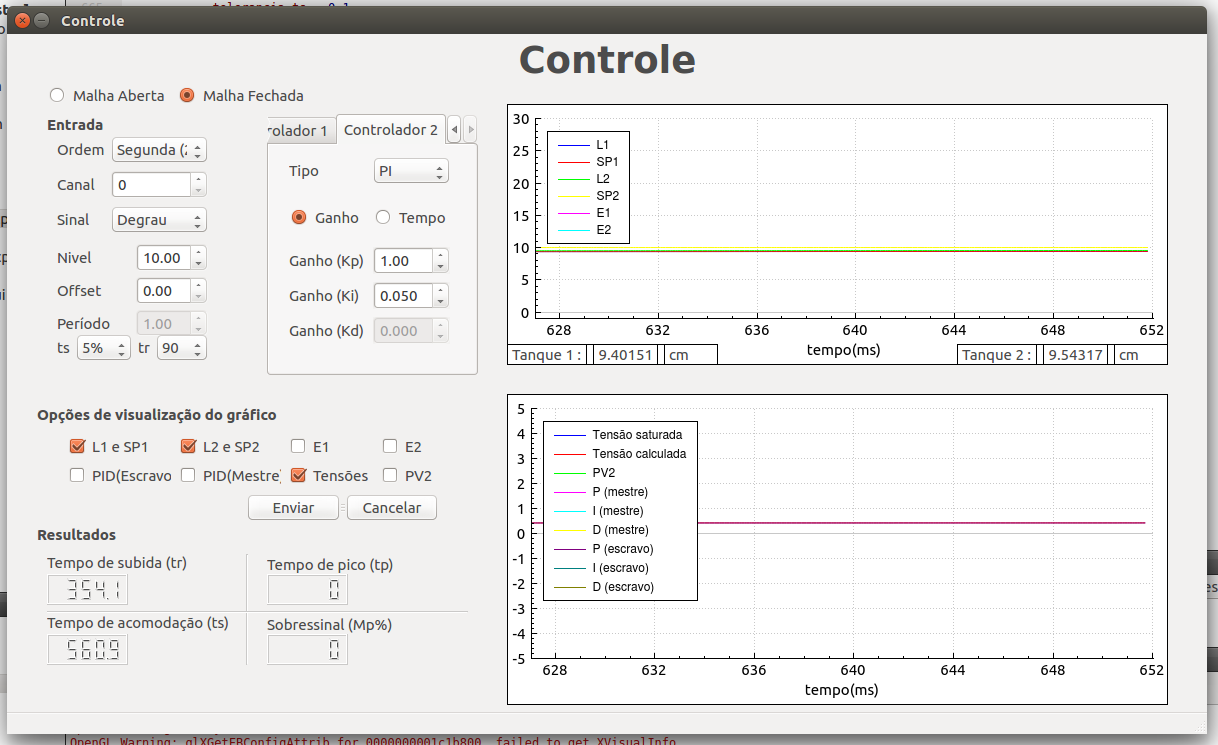
\includegraphics[width=7.4cm]{ImagensLab4/testes/5-1-1.png}\label{img5-1-1}}
\hspace{1cm}
     \subfloat[]{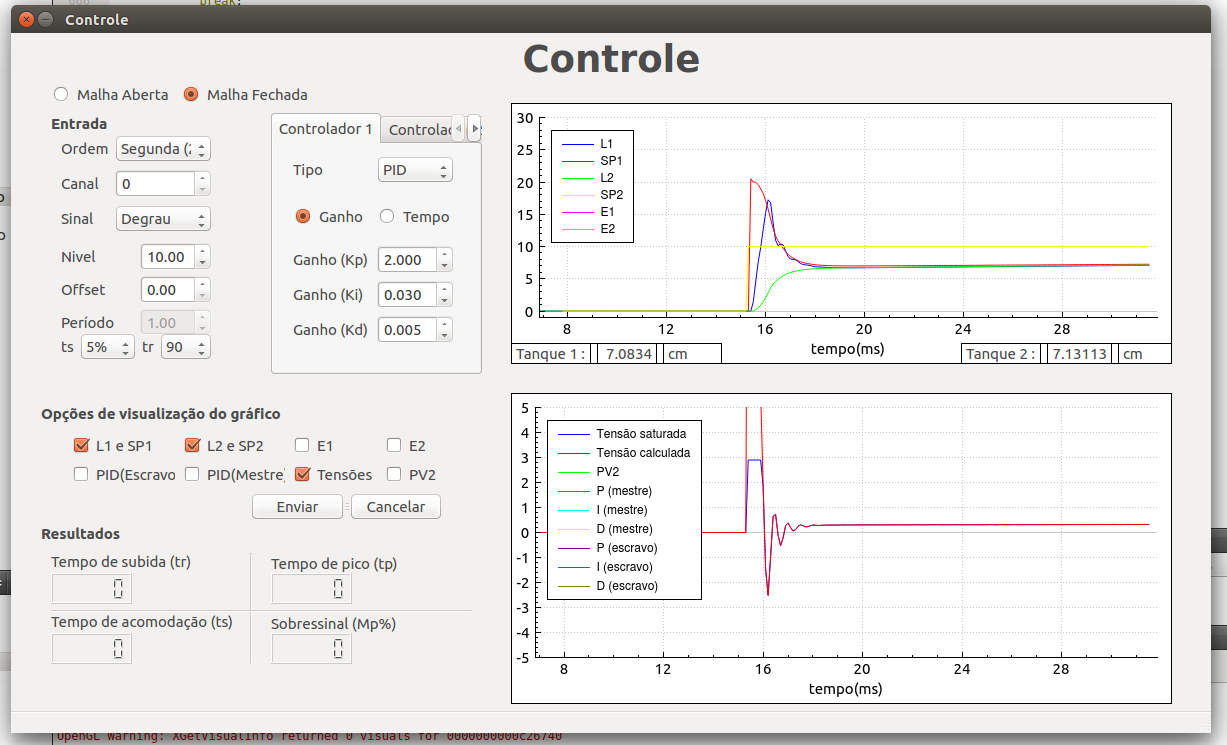
\includegraphics[width=7.4cm]{ImagensLab4/testes/5-0-1.png}\label{img5-2}}
\hspace{1cm}
     \subfloat[]{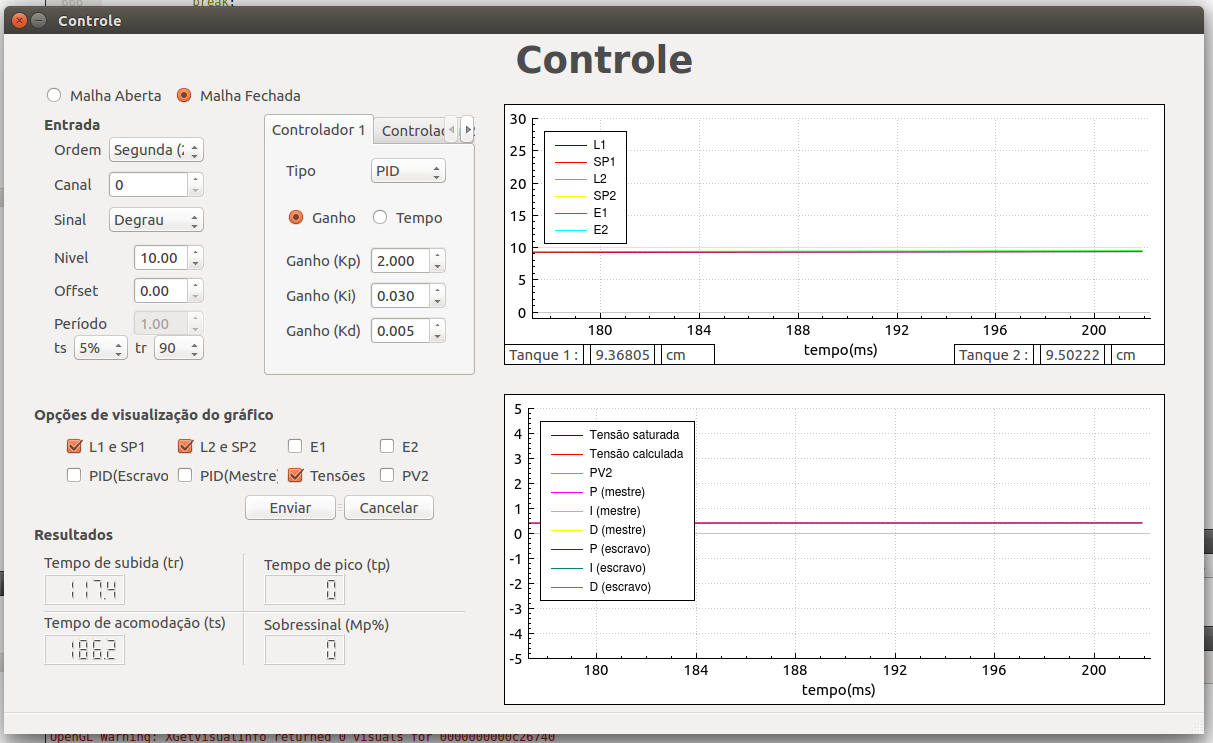
\includegraphics[width=7.4cm]{ImagensLab4/testes/5-0-1-1.png}\label{img5-2-1}}
\hspace{1cm}
     \subfloat[]{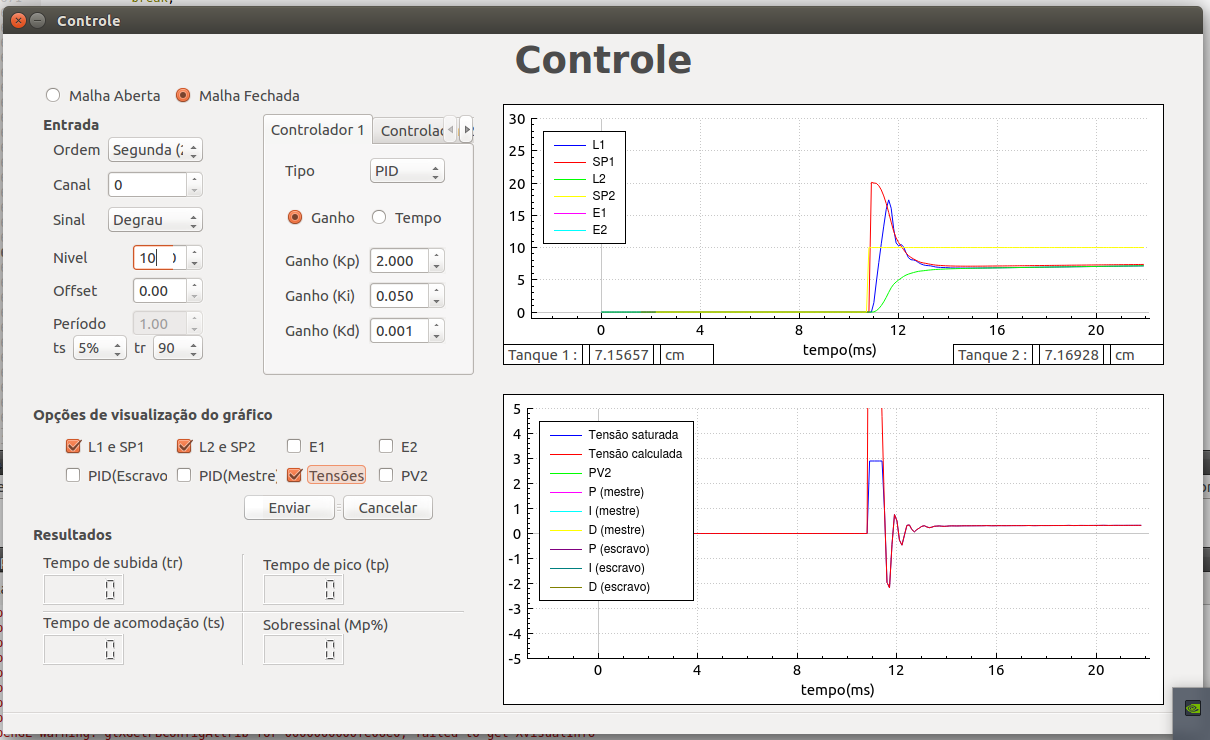
\includegraphics[width=7.4cm]{ImagensLab4/testes/5-0-2.png}\label{img5-3}}
\hspace{1cm}
     \subfloat[]{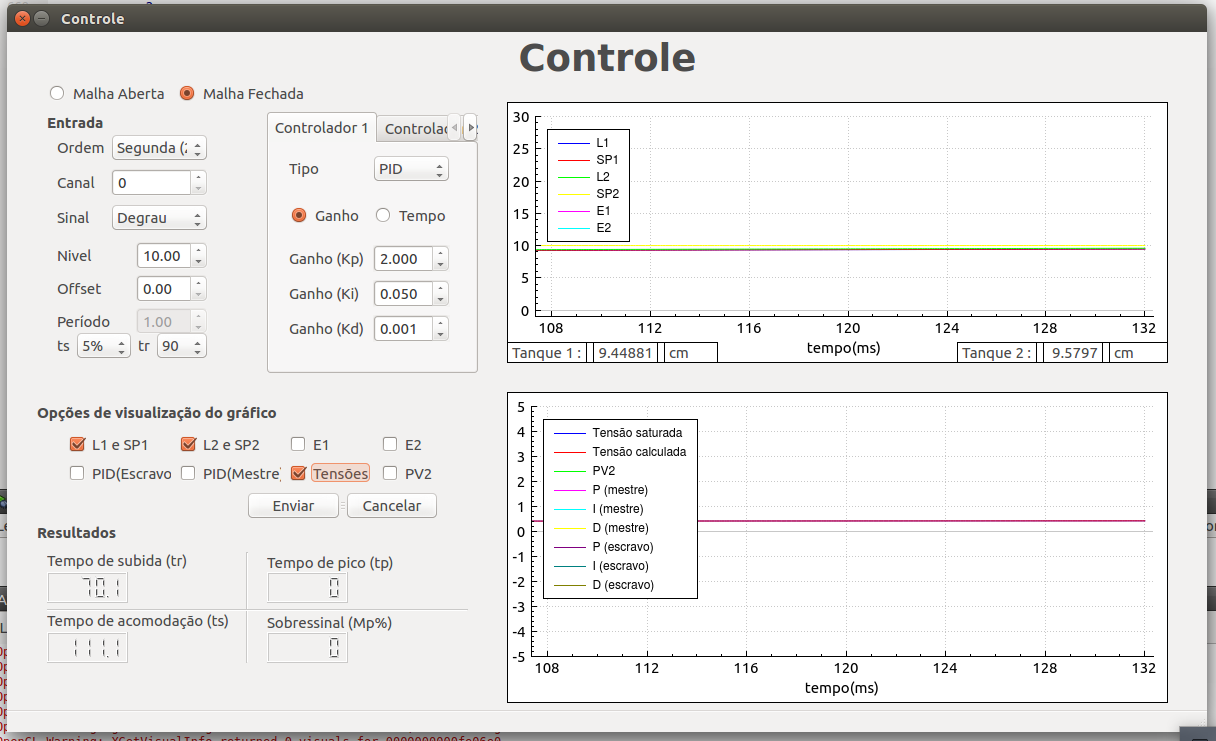
\includegraphics[width=7.4cm]{ImagensLab4/testes/5-0-2-1.png}\label{img5-3-1}}     
     \caption{Controle PID com kp=2 e valores variáveis para ki e kd}
     
\end{figure}

\newpage

%%%%%%%%%% CONCLUSÃO %%%%%%%%%%%%%%%

\thispagestyle{main}

\section{CONCLUSÃO}

\hspace{4ex}Os testes realizados mostram que ao utilizar um controlador em cascata aumenta a estabilidade do sistema diminuindo a sua oscilação do tanque 1 e melhorandado o resultado em geral, mas aumenta a complexidade do projeto pois é necessario sintonizar dois controladores.

\newpage
%%%%%%%% REFERÊNCIAS %%%%%%%%%%%%%%%%%

\thispagestyle{empty}
\section{BIBLIOGRAFIA}

Fundamentals of cascade control | Control Engineering. Disponível em: <http://www.controleng.com/single-article/fundamentals-of-cascade-control/bcedad6518aec409f583ba6bc9b72854.html>. Acesso em: 10 maio. 2017.




%Referências bibliogáficas (geradas automaticamente)

%\addcontentsline{toc}{chapter}{Referências bibliográficas}
%\bibliography{bib/bibliografia}

%\appendix

%Apêndice A
%\include{apendice}

\end{document}
